%include part: see main.beamer.tex and main.article.tex
%include common packages and settings
\usepackage{etex} %эта магическая херь избавляет от переполнения регистров TeX а!!!

\mode<article>{\usepackage{fullpage}}
\mode<presentation>{
    \usetheme{Madrid} %%Boadilla,Madrid,AnnArbor,CambridgeUS,Malmoe,Singapore,Berlin
    \useoutertheme{shadow}
} 

\usepackage[utf8]{inputenc}
\usepackage[russian]{babel}
\usepackage{indentfirst}
\usepackage{graphicx}

\usepackage{amsmath}
\usepackage{amsfonts}
\usepackage{amsthm}
\usepackage{algorithm}
\usepackage{algorithmic}

\usepackage[all]{xy}

\date{Лекция по дисциплине <<дискретная математика>>\\(\today)}
\author[М.~М.~Шихов]{Михаил Шихов \\ \texttt{\underline{m.m.shihov@gmail.com}}}

%для рисования графов пакетом xy-pic
\entrymodifiers={++[o][F-]}

%для псевдокода алгоритмов (algorithm,algorithmic)
\renewcommand{\algorithmicrequire}{\textbf{Вход:}}
\renewcommand{\algorithmicensure}{\textbf{Выход:}}
\renewcommand{\algorithmiccomment}[1]{// #1}
\floatname{algorithm}{Псевдокод}



\title{Основы кодирования}


\begin{document}

%титул и содержание статьи
\mode<article>{\maketitle\tableofcontents}

%титул и содержание презентации
\frame<presentation>{\titlepage}
\begin{frame}<presentation>
    \frametitle{Содержание}
    \tableofcontents
\end{frame}


\begin{frame}
    \frametitle{Определение информации}
    
    \begin{definition}[Юридическое]
        \alert{Информация} --- это сведения (сообщения, данные) независимо от формы их представления\footnote{№149-ФЗ от 27 июля 2006 г <<Об информации, информационных технологиях и о защите информации>>}.
    \end{definition}
    
    \begin{definition}
        \alert{Информация} --- это упорядоченная последовательность (цепочка) \alert{кодовых символов}, принадлежащих конечному алфавиту. При этом каждый символ последовательности несёт определённую смысловую нагрузку.
    \end{definition}
\end{frame}


\begin{frame}
    \frametitle{Свойства информации}

    \begin{center}
        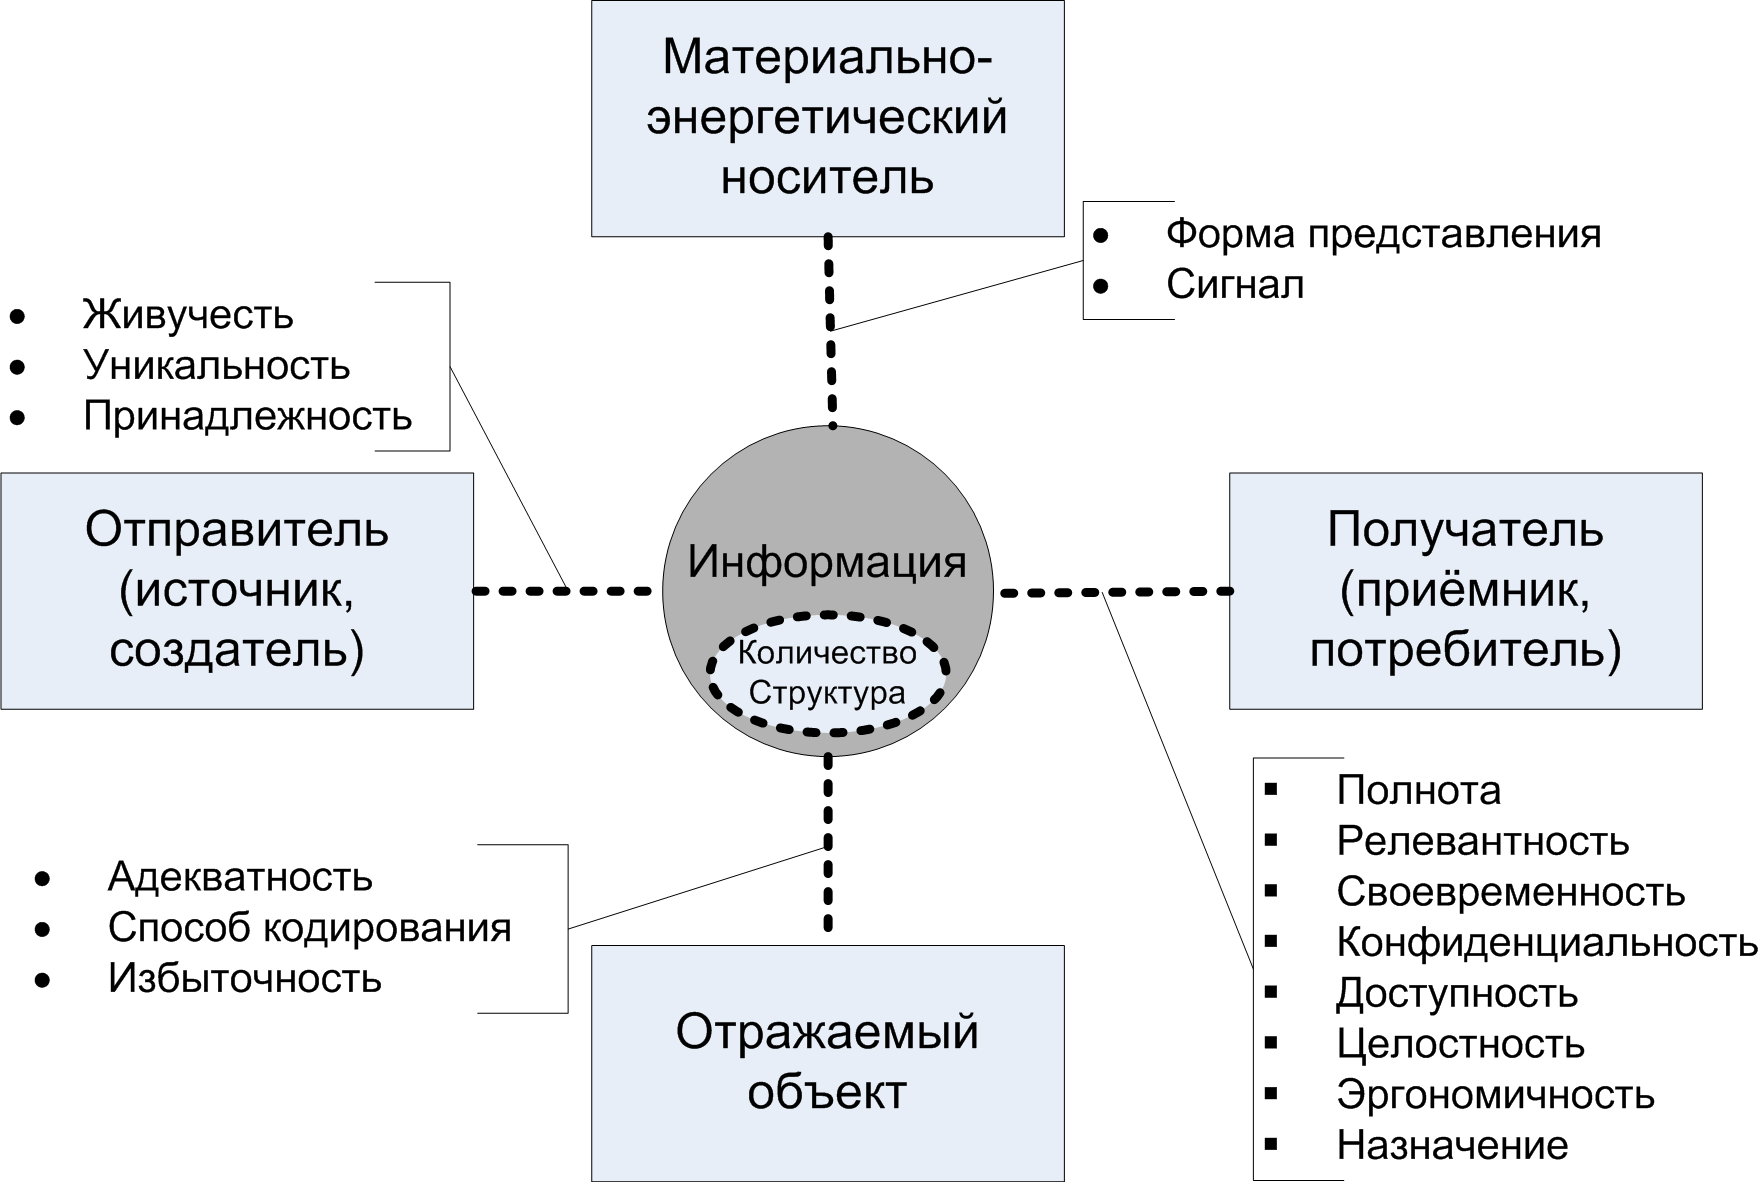
\includegraphics[width=.75\textwidth]{fig/iproperties}
    \end{center}
\end{frame}

\begin{frame}
    \frametitle{Трудности оценки количества информации}

    \begin{itemize}
        \item Просто оценить количество явно заданной информации: достаточно посчитать количество кодовых символов последовательности. 
    
        \item Сложно оценить необходимое количество информации для адекватного <<отражения>> исходного объекта.
    \end{itemize}
\end{frame}

\begin{frame}
    \frametitle{Задача о картах (постановка)}
    
    \begin{example}
        Имеется колода из восьми карт. По две карты (туз и двойка) каждой масти. Некто вытягивает наугад карту и готов честно отвечать только да или нет на любые задаваемые вопросы. Требуется минимальным количеством вопросов угадать вытащенную карту.
    \end{example} 
\end{frame}

\begin{frame}
    \frametitle{Задача о картах (решение)}
    
    \begin{center}
        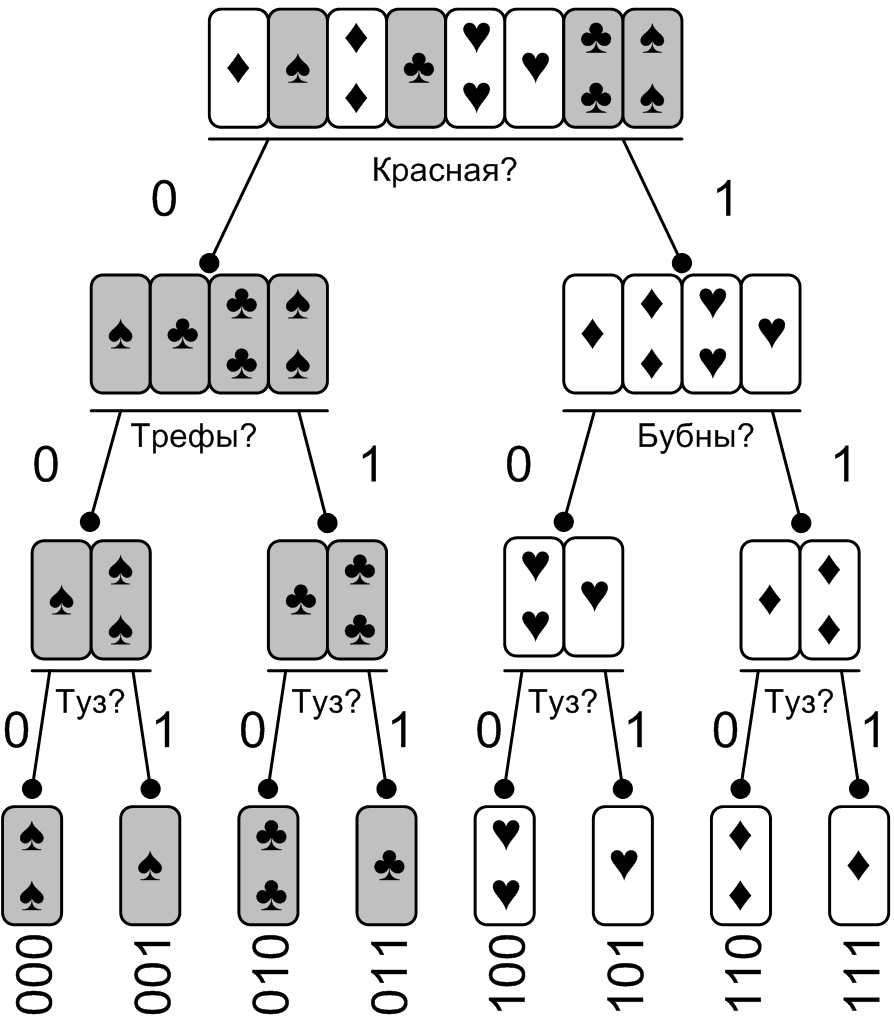
\includegraphics[width=.45\textwidth]{fig/cards} 
    \end{center} 
\end{frame}

\begin{frame}
    \frametitle{Количественная оценка Ральфа Хартли}
    \framesubtitle{$m^H\geq N$}
    
    \[
        H=\log_{m}N,
    \]
    где $m$ --- количество \alert{кодовых символов}; $N$ --- количество состояний \alert{отражаемого объекта}.

    \begin{example}
        В случае примера с картами: количество состояний $N=8$, количество символов $m=2$. Количество информации по Хартли: $H=\log_{2}8=3$ бита.
    \end{example}
\end{frame}

\begin{frame}
    \frametitle{Количественная оценка по Клоду Шеннону}
    \framesubtitle{Постулаты}
    
    Отражаемый объект --- источник \alert{событий}.
    \begin{enumerate}
        \item Количество информации есть непрерывная функция от вероятности события.

        \item Количество информации $I_i$ одиночного $i$-го события $s_i\in S$, $1\leq i\leq N$ происходящего с вероятностью $p_i$, имеет положительное значение. 
        \[I_i\geq 0; I_i=I(p_i); \sum_{i=1}^{N}p_i = 1.\]

        \item Количество информации $I_{ij}$ двух независимых событий $s_i,s_j\in S$ с вероятностью $p_{ij}=p_i\cdot p_j$, равно сумме количеств информаций событий в отдельности:
        \(I_{ij}=I_i+I_j; I(p_i\cdot p_j)=I(p_i) + I(p_j).\)
    \end{enumerate}
\end{frame}

\begin{example}
    Количество воспринимаемой информации влияет на эмоциональное состояние человека и постулаты Шеннона легко проверить на себе.
    
    Согласно Шеннону, количество информации зависит от вероятности наступления события. Сравните свои эмоции от двух событий: <<Жучка укусила Иванова>> и <<Иванов укусил Жучку>>. Первое событие, хоть собака и друг человека, будничное, а вот второе вызывает улыбку --- сенсация! Вероятность первого события весьма велика, вероятность второго близка к нулю. Первое событие несет мало информации, а второе несет большое её количество, отсюда и эмоции.

    В то же время, если мы на следующий день услышим, что после Иванова Жучку укусил еще и Петров, то внутренне мы будем готовы к тому, что на третий день Жучку укусит и Сидоров --- только ленивый не кусает Жучку! Хотя по правилам теории вероятности, с точки зрения обывателя, который не в курсе отношений Жучки с людьми, вероятность того, что Жучку укусит Иванов также мала, как и вероятность быть покусанной Петровым, и равна $p$. Вероятность, того, что Жучка будет покусана обоими, равна произведению вероятностей этих событий: $p^2$ --- это практически невероятно, так как $p^2$ много меньше $p$ и следует ожидать большой сенсации. Но! Никто (разве что Жучка) не падает в обморок от совместных действий Иванова и Петрова, так как количество информации, которое несет данное событие, есть лишь сумма количеств информаций для каждого факта оскорбления действием Жучки в отдельности.
    \qed
\end{example}

\begin{frame}
    \frametitle{Количественная оценка по Клоду Шеннону}
    \framesubtitle{Зависимость информации от вероятности}
    
    \[
        I(p)=-\log_{m}(p),
    \]
    где $I(p)$ --- информация события, происходящего с вероятностью $p$; $m$ --- количество \alert{кодовых символов}.
    
    \begin{example}[$m$ определяет единицы измерения информации]
        \begin{itemize}
            \item $m=2$. \alert{бит}.
            \item $m=e$. \alert{нат}.
            \item $m=3$. \alert{трит}.
            \item $m=10$.\alert{дит}.
        \end{itemize}    
    \end{example}
\end{frame}

\begin{frame}
    \frametitle{Зависимость количества информации от вероятности}
    
    \begin{center}
        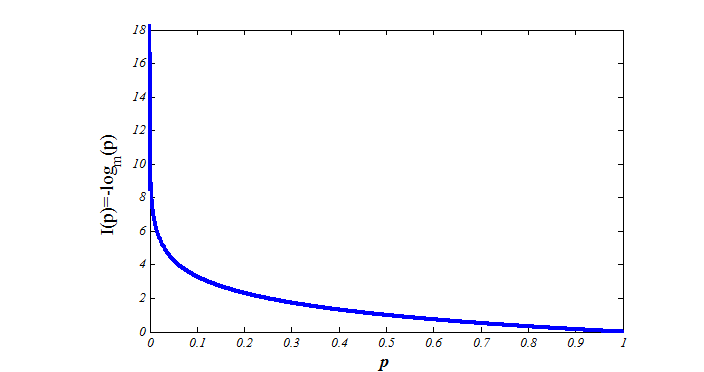
\includegraphics[width=.8\textwidth]{fig/ip}
    \end{center} 
\end{frame}

\begin{frame}
    \frametitle{Задача о биллиардных шарах (постановка)}
    \begin{example}
        Имеется восемь биллиардных шаров с номерами 1-8 соответственно. Все шары одинаковой массы, кроме одного, который тяжелее остальных. Имеются весы Фемиды (чашечные). Какое количество взвешиваний потребуется, чтобы определить номер тяжелого шара?
    \end{example} 
\end{frame}

\begin{frame}
    \frametitle{Задача о биллиардных шарах (решение)}
    \framesubtitle{Решение. $H=\log_{3}9=I(p)=-\log_{3}\frac{1}{9}=2$ трита}
    
    \begin{center}
        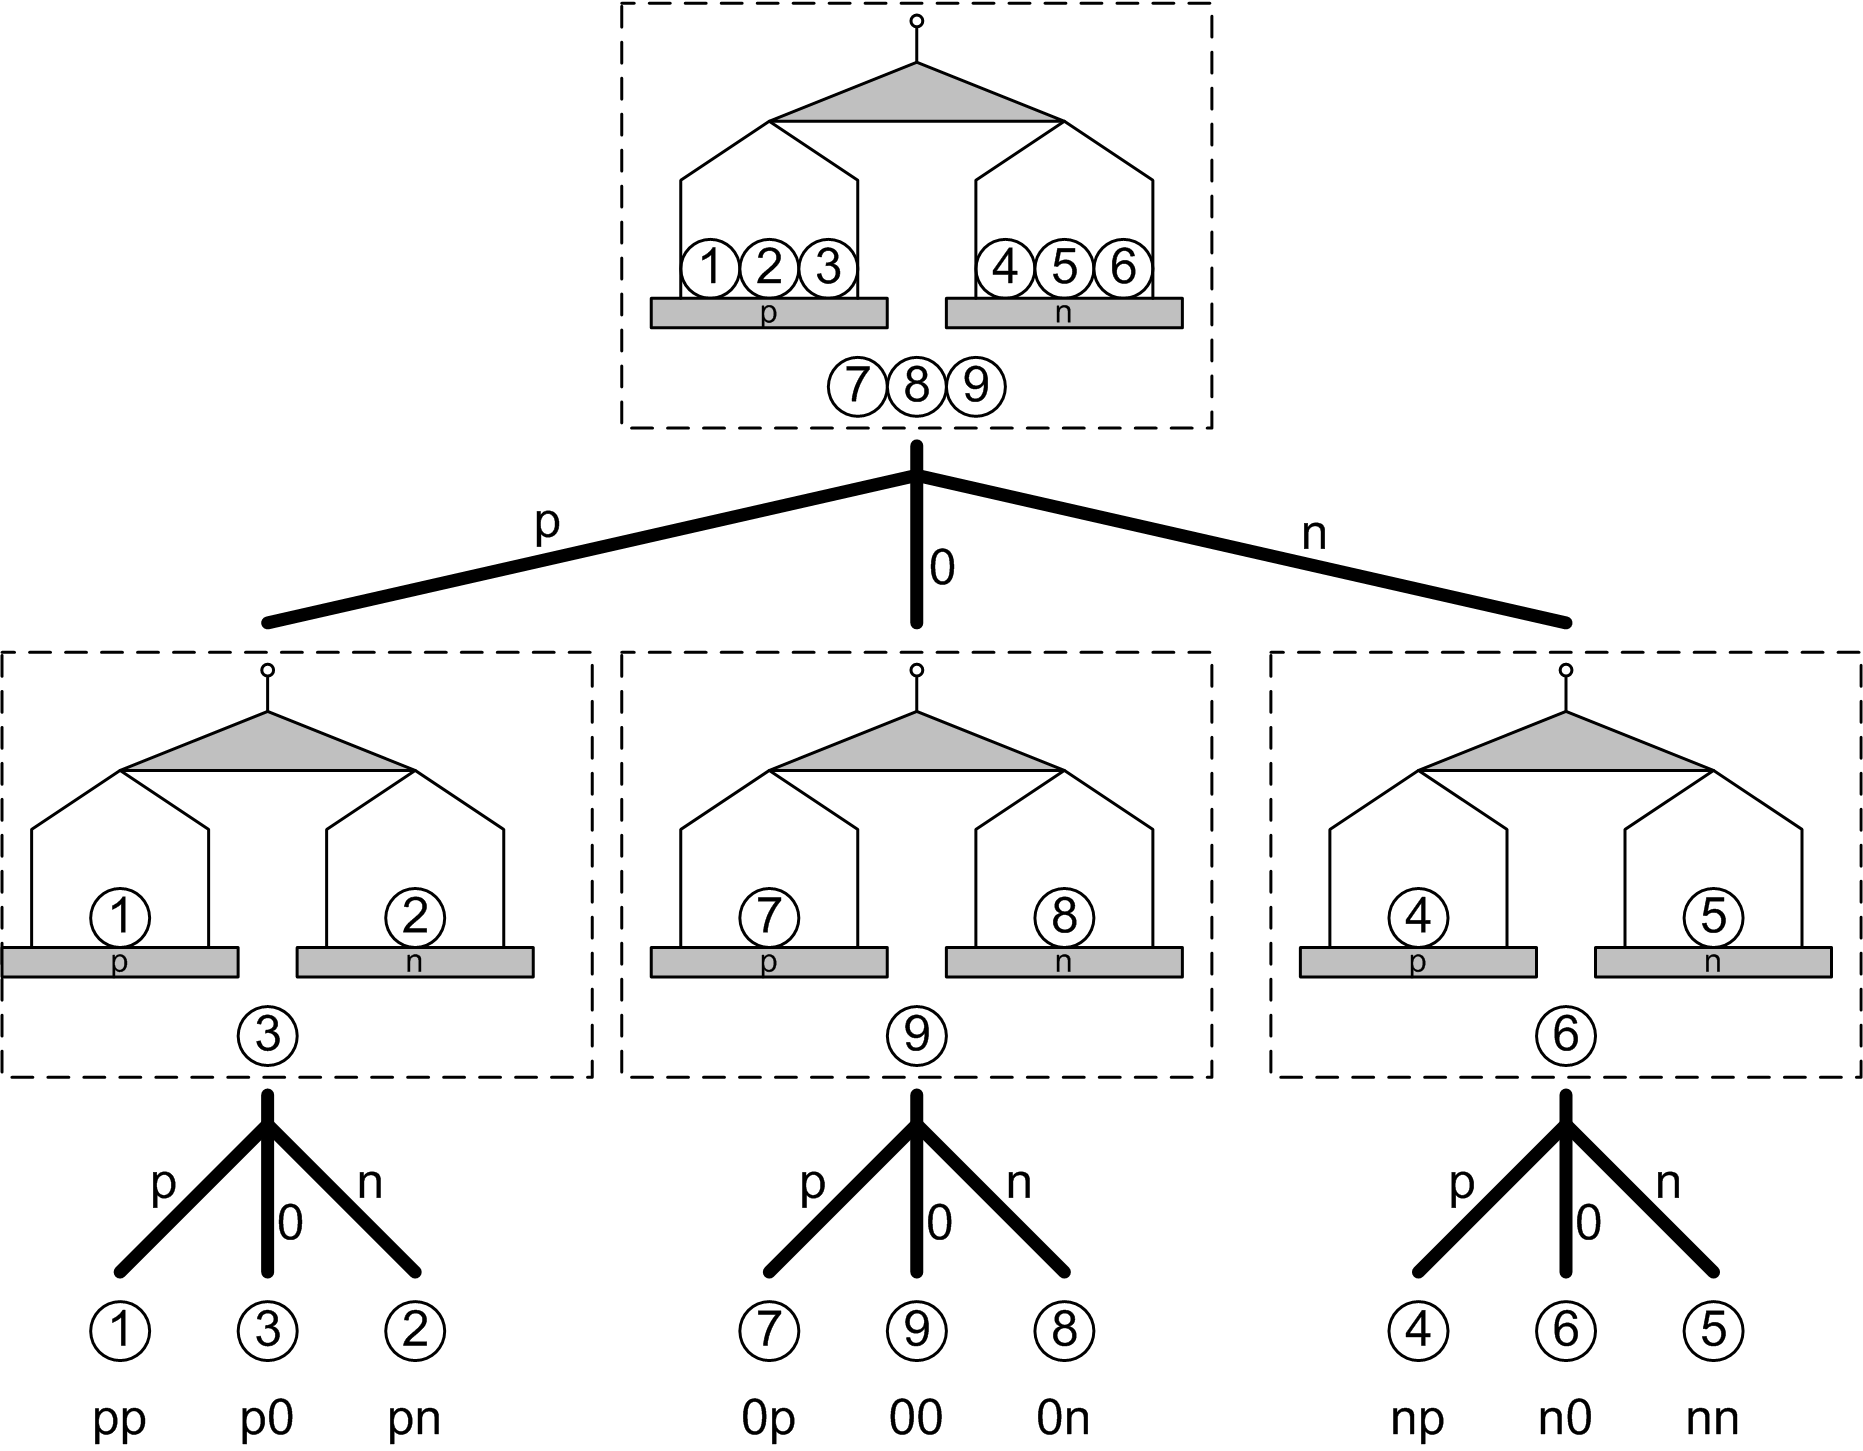
\includegraphics[width=.7\textwidth]{fig/trit}  
    \end{center} 
\end{frame}

\begin{frame}
    \frametitle{Энтропия}
    \framesubtitle{Мера информативности источника событий (сколько выдаёт $I$ в среднем за раз)}
    
    \[
        E=-\sum_{i=1}^{N}p_{i}\cdot \log_{m}p_i.
        \label{eq:e}
    \]
    
    \begin{figure}[!ht]
        \centering
        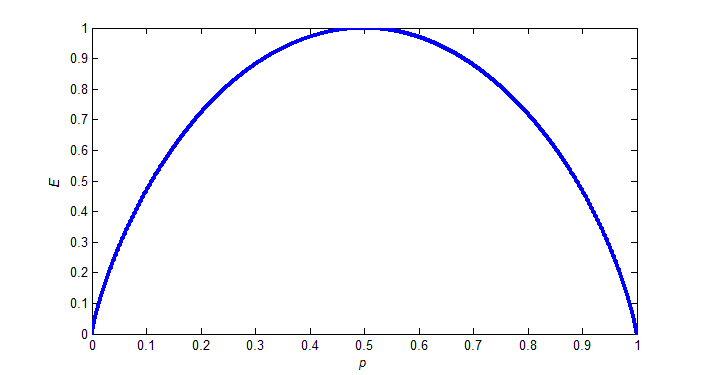
\includegraphics[width=.6\textwidth]{fig/ecoin} 
        \caption{Энтропия для источника с двумя состояниями}\label{pict:ecoin}
    \end{figure} 
\end{frame}

\begin{frame}
    \frametitle{Кодирование}
    
    \begin{definition}
        \alert{Кодирование} --- процесс перехода от \alert{источника событий} к \alert{источнику информации}. Т.е.  сопоставление \alert{событиям} цепочек из \alert{кодовых символов}.
    \end{definition}
    
    Некоторые назначения кодирования:
    \begin{enumerate}
        \item принципиальная возможность описания мира с помощью символов конечного алфавита;
        \item устранение избыточности, сжатие информации, экономия памяти и снижение нагрузки на каналы передачи информации;
        \item обеспечение устойчивости к помехам;
        \item защита важных свойств информации (конфиденциальность, целостность, принадлежность и т.д.).
    \end{enumerate}
\end{frame}

\begin{frame}
    \frametitle{Формальное определение кодирования}
    
    \begin{definition}
        Дано:
        \begin{itemize}
            \item Алфавит \alert{событий}: $S=\{s_1,\ldots,s_N\}$;
            \item Алфавит кодовых \alert{символов}: $T=\{t_1,\ldots,t_m\}$;
        \end{itemize}
        
        Требуется задать отображение $\delta:S\to T^{+}$ (таблицу кодов, \alert{схему кодирования}):
        \[
            \delta=\langle s_1\mapsto \omega_1,\ldots,s_N\mapsto \omega_N\rangle,
        \]
        где $\omega_i=t_{i_1}\cdots t_{i_{k_i}}$, причем слово $\varsigma_j=s_{j_1}\cdots s_{j_t}$ будет кодироваться символами кодового алфавита как $\varsigma_j=\omega_{j_1}\cdots \omega_{j_t}$.
        Множество кодовых слов $\omega_i$, соответствующих $s_i$ называется множеством \alert{элементарных} кодов:
        \[\Omega=\{\omega_1,\ldots,\omega_N\}.\]
    \end{definition} 
\end{frame}

\begin{frame}
    \frametitle{Примеры кодирования}

    \begin{example}[Неоднозначное декодирование. $\delta$ --- не биекция]
        $S=\{A,B,C,D,E,F,G,H\}$; $T=\{0,1\}$; $\delta=\langle A\to 0,B\to 1,C\to 10,D\to 11,E\to 100,F\to 101,G\to 110,H\to 111 \rangle$. 
        \begin{itemize}
            \item Кодирование однозначно: $ABAB\mapsto 0101$. 
            \item Декодирование нет: $0101$ разделяется на слова $ABAB$, $AF$ и $ACB$.
        \end{itemize}
    \end{example} 

    \begin{example}[Однозначное декодирование.  $\delta$ --- биекция]
        $S=\{A,B,C,D,E,F,G,H\}$; $T=\{0,1\}$; $\delta=\langle A\mapsto 000, B\mapsto 001, C\mapsto 010, D\mapsto 011, E\mapsto 100, F\mapsto 101, G\mapsto 110, H\mapsto 111 \rangle$.
        
        \begin{itemize}
            \item Кодирование: $ABBA\mapsto 000111000111$. 
            \item Декодирование: $000111000111\mapsto ABBA$.
        \end{itemize}
    \end{example} 
\end{frame}

\begin{frame}
    \frametitle{Схемы кодирования}

    \begin{definition}
        Схема кодирования $\delta$ является \alert{разделимой}, если любое слово $\varsigma$, составленное из элементарных кодов $\omega_i$ единственным образом разлагается на элементарные коды.
    \end{definition} 
    Разделимая схема допускает декодирование. Важным частным случаем \alert{разделимых} схем являются \alert{префиксные} схемы.
    \begin{definition}
        Схема называется \alert{префиксной}, если ни один элементарный код $\omega_i$ из множества $\Omega$ не является префиксом\footnote{Префиксом слова $\omega$ называется слово $\omega_1$, если $\omega=\omega_1\omega_2$} другого кода из того же множества.
    \end{definition} 
\end{frame}

\begin{frame}
    \frametitle{<<Равномерное>> кодирование}
    
    Наиболее простым вариантом кодирования является \alert{равномерное} кодирование, когда все элементарные коды равной длины.
    
    Для кодирования $N$ событий требуется использовать цепочки длины
    \[
        I(n)=\lceil\log_m(n)\rceil,
    \]
    где $m$ --- количество кодовых символов; $\lceil X \rceil$ --- наименьшее целое, большее или равное $X$.
    
    Эта же оценка на основе постулатов Шеннона:
    \[
        I(n)=\left\lceil -\log_m\left(\frac{1}{n}\right) \right\rceil=\lceil \log_m(n) \rceil.
    \]
\end{frame}

\begin{frame}
    \frametitle{Равномерное кодирование}

    \begin{example}
        В соревновании учавствуют $33$ спортсмена. Для регистрации пересечения финишной черты каждому спортсмену выдается радио-брелок. В момент пересечения финишной черты спортсменом, брелок передает двоичный код для идентификации спортсмена. Все брелки передают код одинаковой длины. Какое минимально необходиоме количество бит в общем случае должен передать брелок?
    \end{example}
    \begin{proof}<2>[Решение] 
        $\lceil \log_2(33)\rceil = 6$.
    \end{proof}
\end{frame}

В ряде случаев в процессе кодирования имеются знания о вероятности возникновения тех или иных событий. Если это так, то можно использовать методики оптимального кодирования для экономии памяти (или снижения нагрузки на каналы передачи данных).


\section{Оптимальное кодирование}

\subsection{Энтропия}

\begin{frame}
    \frametitle{Информативность источника \alert{событий}}
    
    Источнику событий после кодирования соответствует источник информации, выдающий коды событий. Оценку информативности \alert{источника событий} дает величина, называемая \alert{энтропией} источника событий:
    \begin{equation}
        \label{eq:code:entrophyS}
        E=-\sum_{i=1}^N {p_i\cdot\log_m p_i},
    \end{equation}
    где $p_i$ --- вероятность $i$-го события $s_i\in S$ на выходе источника событий, $m$ --- количество кодовых символов, $N$ --- количество событий $N=|S|$.
\end{frame}

\begin{frame}
    \frametitle{Информативность источника \alert{информации}}
    
    Так как вероятности появления кодов событий останутся прежними, то энтропия \alert{источника информации} $E'$ будет равна
    \begin{equation}
        \label{eq:code:entrophyI}
        E'=\sum_{i=1}^n {p_i\cdot I_i},
    \end{equation}
    где $I_i$ --- длина кода $\omega_i$ для $i$-го события.
    
    \begin{center}
        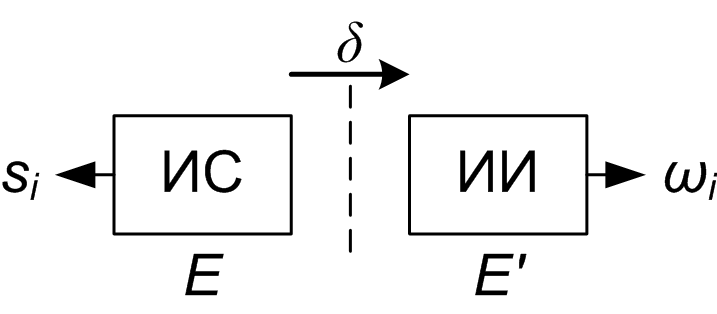
\includegraphics[width=.5\textwidth]{fig/reflection}
    \end{center}
\end{frame}

\begin{frame}
    \frametitle{Задача оптимального кодирования}
    
    \begin{block}{Аксиома}
        Энтропия источника информации всегда больше энтропии отражаемого источника событий. 
    \end{block}
    Задача оптимального кодирования: максимально приблизить энтропию источника информации к энтропии источника событий.
\end{frame}

\begin{frame}
    \frametitle{Оценка оптимальности кодирования}
    
    Пусть имеется источник событий $s_i$, о вероятности появления которых на его выходе известно следующее:
    
    \begin{center}
        \begin{tabular}{|l|c|c|c|c|}
            \hline
            Событие $s_i$                   &А      &Б      &В      &Г   \\ \hline
            Вероятность $p_i$ события $s_i$ &0.5    &0.3    &0.1    &0.1 \\ \hline
        \end{tabular}
    \end{center}
    
    Энтропия источника событий, формула \eqref{eq:code:entrophyS}, составляет:
    \[
        \begin{split}
            E=-(0.5\cdot\log_2 0.5+0.3\cdot\log_2 0.3+0.1\cdot log_2 0.1+0.1\cdot log_2 0.1)\approx \\
            \approx(0.5+0.521089678+0.332192809+0.332192809)\approx \\
            \approx 1.685475297\text{ бит}.
        \end{split}
    \]
\end{frame}

\begin{frame}
    \frametitle{Оценка оптимальности кодирования}
    
    Для равномерного кодирования битами может быть получен такой вариант:

    \begin{center}
        \begin{tabular}{|l|c|c|c|c|}
            \hline
            Событие $s_i$                   &А      &Б      &В      &Г   \\ \hline
            Вероятность $p_i$ события $s_i$ &0.5    &0.3    &0.1    &0.1 \\ \hline
            Код события $\omega_i$          &00     &01     &10     &11  \\ \hline
        \end{tabular}
    \end{center}
    
    Энтропия данного источника информации составит, по формуле \eqref{eq:code:entrophyI}:
    \[
        E'=(0.5\cdot 2+0.3\cdot 2+0.1\cdot 2+0.1\cdot 2)=2 \text{ бита}.
    \]
\end{frame}
    
Видно, что энтропия источника информации значительно больше. Можно ли её уменьшить, приблизить к энтропии источника событий? Очевидно, что если кодировать символы с большей вероятностью появления кодом с меньшей длиной, то результаты должны получиться лучше. Попробуем следующую схему:
    
\begin{frame}
    \frametitle{Оценка оптимальности кодирования}
    
    \begin{center}
        \begin{tabular}{|l|c|c|c|c|}
            \hline
            Событие $s_i$                   &А      &Б      &В      &Г   \\ \hline
            Вероятность $p_i$ события $s_i$ &0.5    &0.3    &0.1    &0.1 \\ \hline
            Код события $\omega_i$          &0      &10     &110    &111 \\ \hline
        \end{tabular}
    \end{center}
    
    Так же как и предыдущая, эта схема префиксная и разделимая, но неравномерная. Энтропия источника информации теперь составляет
    \[
        E'=(0.5\cdot 1+0.3\cdot 2+0.1\cdot 3+0.1\cdot 3)=1.7\text{ бита}.
    \]
\end{frame}

\begin{frame}
    \frametitle{Оценка оптимальности кодирования}
    
    Представленные источники \alert{эквивалентны}. Если запустить источник информации на выдачу, например, $100$ кодов событий, то первый вариант кодирования выдаст цепочку длины $\approx 200$, а второй --- $\approx 170$ бит.
\end{frame}

Далее рассматриваются два алгоритма оптимального кодирования источника событий: алгоритм Хаффмана и алгоритм Фано. 


\subsection{Алгоритм Хаффмана для $m=2$}

\begin{frame}
    \frametitle{Алгоритм Хаффмана для $m=2$}
    
    \begin{enumerate}
        \item\label{enum:code:haffSort} 
        События сортируются по убыванию вероятности.
        
        \item\label{enum:code:haffGlue} 
        Два события с минимальными вероятностями объединяются в одно составное событие c суммарной вероятностью исходных. При этом одно из исходных событий помечается кодовым символом $0$, а второе --- символом $1$. Исходные события исключаются из множества событий, вместо них остается одно составное.
        
        \item Шаги \ref{enum:code:haffSort} и \ref{enum:code:haffGlue} последовательно повторяются до тех пор, пока все события не склеятся в единственное составное событие, вероятность которого равна $1$. После этого кодовое слово $\omega_i$ для исходного события $s_i$ есть цепочка из кодовых символов, которыми помечены все составные события от  корня до $s_i$.
    \end{enumerate}
\end{frame}

\begin{frame}
    \frametitle{Оптимальное кодирование по Хаффману}
    
    \begin{center}
        \begin{tabular}{|l|c|c|c|c|}
            \hline
            Событие $s_i$                   &А      &Б      &В      &Г   \\ \hline
            Вероятность $p_i$ события $s_i$ &0.5    &0.3    &0.1    &0.1 \\ \hline
            Код события $\omega_i$          &\uncover<6>{0}      
                                                    &\uncover<6>{10}     
                                                            &\uncover<6>{110}    
                                                                    &\uncover<6>{111} 
                                                                         \\ \hline
        \end{tabular}
    \end{center}
    \begin{center}
        \only<1>{ 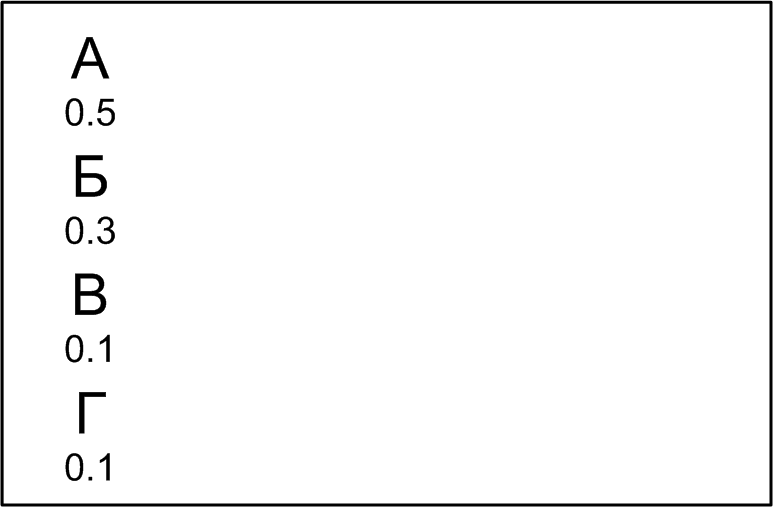
\includegraphics[width=0.6\textwidth]{fig/huffmanX1} }
        \only<2>{ 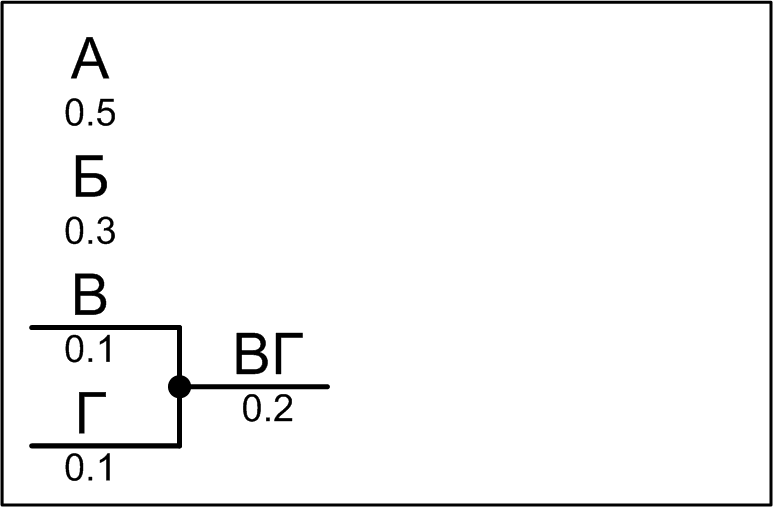
\includegraphics[width=0.6\textwidth]{fig/huffmanX2} }
        \only<3>{ 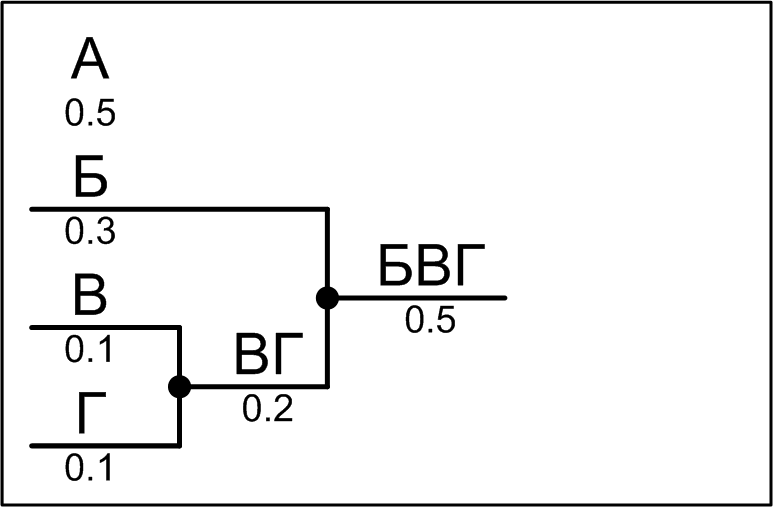
\includegraphics[width=0.6\textwidth]{fig/huffmanX3} }
        \only<4>{ 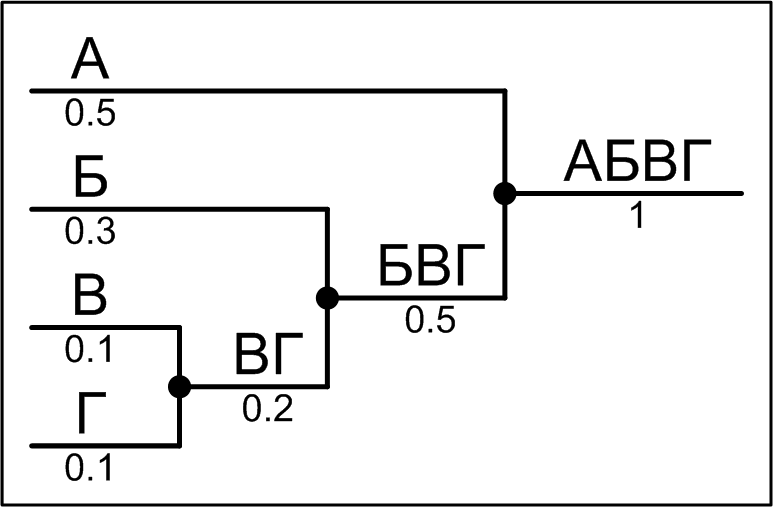
\includegraphics[width=0.6\textwidth]{fig/huffmanX4} }
        \only<5->{ 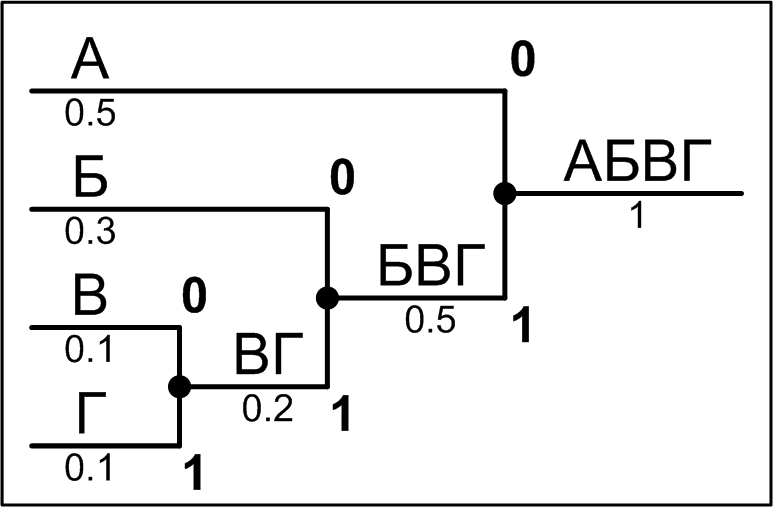
\includegraphics[width=0.6\textwidth]{fig/huffmanXE} }
    \end{center}
\end{frame}


\begin{frame}
    \frametitle{Оптимальное кодирование по Хаффману (задача)}
    
    \begin{center}
        \begin{tabular}{|l|c|c|c|c|c|}
            \hline
            Событие $s_i$                   &А      &Б      &В      &Г      &Д      \\ \hline
            Вероятность $p_i$ события $s_i$ &0.5    &0.125  &0.125  &0.125  &0.125  \\ \hline
            Код события $\omega_i$          &\uncover<2->{0} 
                                                    &\uncover<2->{100}    
                                                            &\uncover<2->{101}    
                                                                    &\uncover<2->{110}    
                                                                            &\uncover<2->{111}    
                                                                                    \\ \hline
        \end{tabular}
    \end{center}
    \uncover<2->{
        \begin{center}
            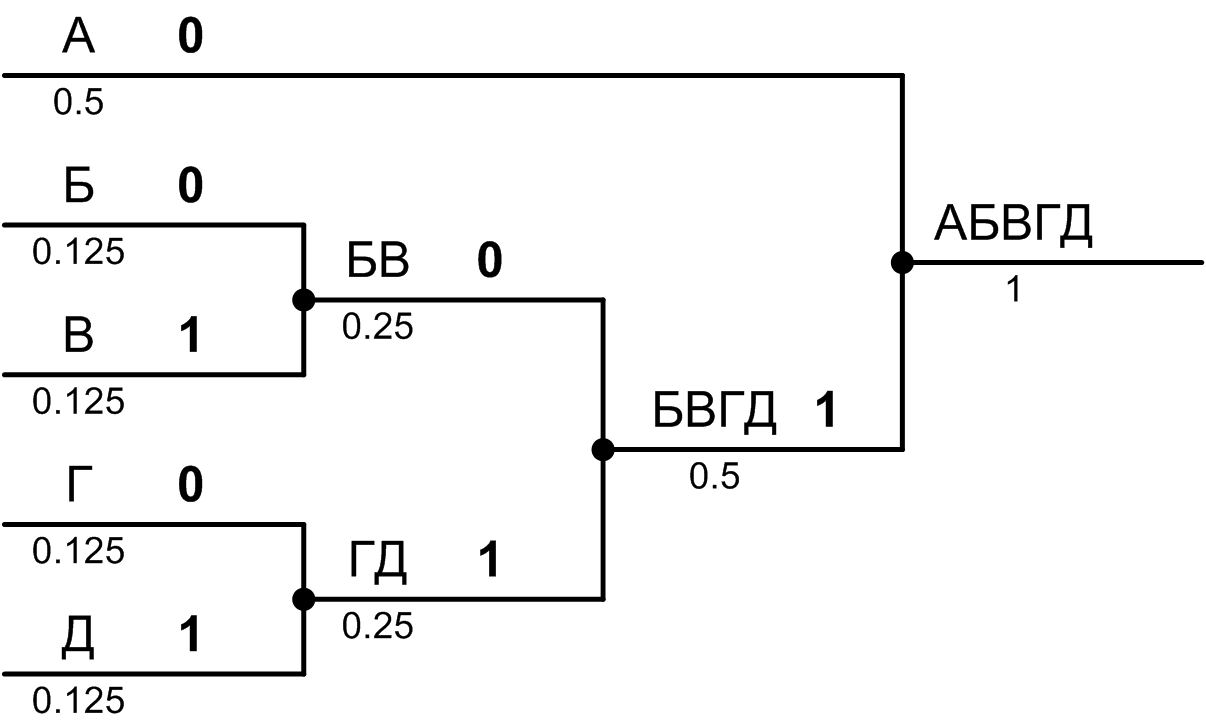
\includegraphics[width=0.6\textwidth]{fig/haffman2Ex}
        \end{center}
    }    
    \uncover<2->{$10001101110111\to\uncover<3->{\text{БАГДАД}}$}
\end{frame}


\subsection{Алгоритм Фано для $m=2$}

\begin{frame}
    \frametitle{Алгоритм Фано для $m=2$}
    
    \begin{enumerate}
        \item Исходный массив событий, сортируется в порядке убывания вероятностей. 
    
        \item \label{en:code:fanoSplit} Массив разбивается на две части, так, чтобы разница сумм вероятностей событий каждой части была минимальна. Первый кодовый символ элементарного кода $\omega_i$ находится так: для всех событий левой части разбитого массива кодовый символ будет $0$, а для всех событий правой части --- $1$. 
    
        \item Второй и последующие кодовые символы определяется так: каждая часть разбитого исходного массива, в которой более одного события, становится исходным массивом, и её разбиение выполняется так же, как исходного массива (шаг \ref{en:code:fanoSplit}).
    \end{enumerate}
\end{frame}

\begin{frame} 
    \frametitle{Оптимальное кодирование по алгоритму Фано}

    \begin{center}
        \begin{tabular}{|l|c|c|c|c|}
            \hline
            Событие $s_i$                   &А      &Б      &В      &Г   \\ \hline
            Вероятность $p_i$ события $s_i$ &0.5    &0.3    &0.1    &0.1 \\ \hline
            Код события $\omega_i$          &\uncover<5>{0}      
                                                    &\uncover<5>{10}     
                                                            &\uncover<5>{110}    
                                                                    &\uncover<5>{111} 
                                                                         \\ \hline
        \end{tabular}
    \end{center}
    
    \only<1>{
        \begin{center}
            \begin{tabular}{|l|l||}
                \hline\hline
                $s_i$   &$p_i$  \\ \hline\hline
                А       &0.5    \\
                Б       &0.3    \\
                В       &0.1    \\
                Г       &0.1    \\ \hline
            \end{tabular}
        \end{center}
    }
    \only<2>{
        \begin{center}
            \begin{tabular}{|l|l||c}
                \hline\hline
                $s_i$   &$p_i$  &\multicolumn{1}{c}{$\omega_i$} \\ \hline\hline
                А       &0.5    &0                              \\ \cline{3-3}
                Б       &0.3    &1                              \\ 
                В       &0.1    &1                              \\ 
                Г       &0.1    &1                              \\ \hline
            \end{tabular}
        \end{center}
    }
    \only<3>{
        \begin{center}
            \begin{tabular}{|l|l||c|c}
                \hline\hline
                $s_i$   &$p_i$  &\multicolumn{2}{c}{$\omega_i$} \\ \hline\hline
                А       &0.5    &0&\multicolumn{1}{c}{}         \\ \cline{3-4}
                Б       &0.3    &1&0                            \\ \cline{4-4}
                В       &0.1    &1&1                            \\ 
                Г       &0.1    &1&1                            \\ \hline
            \end{tabular}
        \end{center}
    }
    \only<4->{
        \begin{center}
            \begin{tabular}{|l|l||c|c|c|}
                \hline\hline
                $s_i$   &$p_i$  &\multicolumn{3}{c|}{$\omega_i$} \\ \hline\hline
                А       &0.5    &0&\multicolumn{2}{c|}{}         \\ \cline{3-4}
                Б       &0.3    &1&0&\multicolumn{1}{c|}{}       \\ \cline{4-5}
                В       &0.1    &1&1&0                           \\ \cline{5-5}
                Г       &0.1    &1&1&1                           \\ \hline
            \end{tabular}
        \end{center}
    }    
\end{frame}

\begin{frame} 
    \frametitle{Оптимальное кодирование по алгоритму Фано (задача)}

    \begin{center}
        \begin{tabular}{|l|c|c|c|c|c|c|c|c|}
            \hline
            $s_i$       &А      &Б      &В      &Г      &Д      &Е      &Ж      \\ \hline
            $p_i$       &0.135  &0.24   &0.25   &0.125  &0.0635 &0.124  &0.0625 \\ \hline
            $\omega_i$  &\uncover<3->{100}  
                                &\uncover<3->{01}   
                                        &\uncover<3->{00}   
                                                &\uncover<3->{101}  
                                                        &\uncover<3->{1110} 
                                                                &\uncover<3->{110}  
                                                                        &\uncover<3->{1111} 
                                                                                \\ \hline
        \end{tabular}
    \end{center}
    
    \uncover<2->{
        \begin{center}
            \begin{tabular}{|l|l||c|c|c|c|}
                \hline\hline
                $s_i$   &$p_i$  &\multicolumn{4}{c|}{$\omega_i$}\\ \hline\hline
                В       &0.25   &0&0&\multicolumn{2}{c|}{}      \\ \cline{4-4}
                Б       &0.24   &0&1&\multicolumn{2}{c|}{}      \\ \cline{3-5}
                А       &0.135  &1&0&0&                         \\ \cline{5-5}
                Г       &0.125  &1&0&1&                         \\ \cline{4-5}
                Е       &0.124  &1&1&0&                         \\ \cline{5-6}
                Д       &0.0635 &1&1&1&0                        \\ \cline{6-6}
                Ж       &0.0625 &1&1&1&1                        \\ \hline            
            \end{tabular}
        \end{center}
    }
\end{frame}


\section{Кодирование с целью сжатия информации}

Следует выделить различия между между \emph{оптимальным кодированием} и \emph{кодированием с целью сжатия}? Оптимальное кодирование ставит себе в задачу сопоставить источнику событий минимальное количество адекватной ему информации. 


\subsection{Сжатие}

\begin{frame}
    \frametitle{Сжатие}
    
    Кодирование с целью сжатия (или просто \alert{сжатие}) ставит себе в задачу уменьшить количество информации, не теряя (или оставаясь в допустимых рамках) при этом свойство адекватности отражаемому объекту. В случае сжатия, события $s_i$ уже представляют собой слова в алфавите $T$ (коды). При сжатии информация \alert{перекодируется} в том же алфавите $T$.
    
    Классы алгоритмов сжатия:
    \begin{itemize}
        \item сжатие с потерями (адекватности);
        \item сжатие без потерь.
    \end{itemize}
\end{frame}

Выделяют два больших класса алгоритмов сжатия информации: сжатие с потерями и без потерь. Теряется, данном случае, конечно, адекватность отражения. При сжатии без потерь из сжатой информации можно восстановить исходную информацию в точности такую же, как до сжатия. При сжатии с потерями восстановленная информация будет отличаться от исходной. Ярким примером сжатия с потерями является сжатие изображений: используя определенные особенности восприятия цвета человеком, такие алгоритмы отбрасывают <<лишнюю>> информацию. Потеря адекватности отражаемому объекту в этом случае значительная, но для человека-потребителя эти потери адекватности незаметны.

Часто алгоритмы сжатия весьма специфичны и учитывают особенности отражаемого источника событий. Одним из важнейших таких источников в жизни человека является речь. Письмо --- способ кодирования речи с помощью символов конечного алфавита --- азбуки. На основе, например, русского алфавита можно построить бесконечное количество слов, но в реальной жизни словарный запас редко превышает сотню тысяч слов. На практике для универсального представления текста байтами кодируются буквы, цифры, знаки препинания, пробелы и т.д., но если мы знаем, что кодируется именно осмысленный текст (содержащий осмысленные слова), то можно сильно сэкономить, кодируя в качестве сообщений $s_i$ не буквы, а слова. Такие методы сжатия называются \emph{словарными}. 

Впрочем, словарные методы могут использоваться не только для кодирования текста, но для произвольных информационных цепочек. Причем словарь может строиться динамически и совершенно не учитывать смысловой нагрузки слов в словаре.

Далее будет рассмотрен алгоритм Лемпела-Зива, относящийся к группе словарных. В основе алгоритма Лемпела-Зива лежит идея \emph{адаптивного} сжатия: за один проход по цепочке одновременно строится и словарь и код, причем словарь не хранится, так как при декодировании он динамически восстанавливается.


\subsection{Алгоритм Лемпела-Зива}

\begin{frame}
    \frametitle{Алгоритм Лемпела-Зива (LZ)}
    \framesubtitle{Кодирование}
    
	\begin{enumerate}
		\item В словарь нулевым элементом помещается пустая цепочка $\varepsilon$. Пустое слово $\varepsilon$ не содержит букв, и для любого слова $\omega$ справедливо $\omega=\varepsilon\omega=\omega\varepsilon$.
        
        \item\label{enum:code:lzWord} От исходной цепочки $t$ отделяется слово $\omega a$, где $\omega$ --- максимально длинное слово из словаря, $a$ --- расширяющая буква. Т.е. $t=\omega at'$.
        
        \item\label{enum:code:lzDict} В конец словаря добавляется новое слово $\omega a$. К коду $c$ добавляется пара $\langle i_{\omega},a\rangle$, где $i_{\omega}$ --- индекс слова $\omega$ в словаре. От исходного текста отделяется слово $\omega a$: $t=t'$.
        
        \item Пункты \ref{enum:code:lzWord}-\ref{enum:code:lzDict} последовательно повторяются до тех пор, пока в тексте $t$ остается хоть одна буква.
	\end{enumerate}
    В результате получается код $c=\langle i_1,a_1\rangle\cdots\langle i_n,a_n\rangle$.
\end{frame}

Нужно отметить, что данный алгоритм хорошо сжимает тексты большого объема, в которых так или иначе будут присутствовать одинаковые и достаточно длинные слова. В следующем примере такие вхождения были созданы искусственно.

\begin{frame}
    \frametitle{Алгоритм Лемпела-Зива}
    \framesubtitle{Пример сжатия текста: <<АБАКАНКАНКАНКИАНКИН>>}
    
    \begin{center}
        \resizebox{.8\textwidth}{!}{
            \begin{tabular}[c]{|l|l|l|l|}
            \hline\hline
            $i$ & $t$                                            & $\omega a$                   & $c=\langle i_\omega,a\rangle$ \\ 
            \hline\hline
              &                                                  & $0\rightarrow\varepsilon $   & \\ \hline
            1 &	$\varepsilon\text{\textbf{А}БАКАНКАНКАНКИАНКИН}$ & $1\rightarrow\text{A}    $   & $\langle\text{0,А}\rangle$ \\ \hline
            2 &	$\varepsilon\text{\textbf{Б}АКАНКАНКАНКИАНКИН} $ & $2\rightarrow\text{Б}    $   & $\langle\text{0,Б}\rangle$ \\ \hline
            3 &	$           \text{\textbf{АК}АНКАНКАНКИАНКИН}  $ & $3\rightarrow\text{АК}   $   & $\langle\text{1,К}\rangle$ \\ \hline
            4 &	$           \text{\textbf{АН}КАНКАНКИАНКИН}    $ & $4\rightarrow\text{АН}   $   & $\langle\text{1,Н}\rangle$ \\ \hline
            5 &	$\varepsilon\text{\textbf{К}АНКАНКИАНКИН}      $ & $5\rightarrow\text{К}    $   & $\langle\text{0,К}\rangle$ \\ \hline
            6 &	$           \text{\textbf{АНК}АНКИАНКИН}       $ & $6\rightarrow\text{АНК}  $   & $\langle\text{4,К}\rangle$ \\ \hline
            7 &	$           \text{\textbf{АНКИ}АНКИН}          $ & $7\rightarrow\text{АНКИ} $   & $\langle\text{6,И}\rangle$ \\ \hline
            8 &	$           \text{\textbf{АНКИН}}              $ & $8\rightarrow\text{АНКИН}$   & $\langle\text{7,Н}\rangle$ \\ \hline
            \end{tabular}
        }        
    \end{center}
    \[
        \overbrace{\varepsilon}^0
        \overbrace{\text{А}}^1_{\langle 0,\text{А}\rangle}
        \overbrace{\text{Б}}^2_{\langle 0,\text{Б}\rangle}
        \overbrace{\text{АК}}^3_{\langle 1,\text{К}\rangle}
        \overbrace{\text{АН}}^4_{\langle 1,\text{Н}\rangle}
        \overbrace{\text{К}}^5_{\langle 0,\text{К}\rangle}
        \overbrace{\text{АНК}}^6_{\langle 4,\text{К}\rangle}
        \overbrace{\text{АНКИ}}^7_{\langle 6,\text{И}\rangle}
        \overbrace{\text{АНКИН}}^8_{\langle 7,\text{Н}\rangle}
    \]
    
    Дать оценку длин кода и текста
\end{frame}

Полученный код (сжатый текст) занимает 8*2=16 байт информации (один байт на индекс, второй на букву), а код исходного текста занимает 19 байт (один байт на букву).

\begin{frame}
    \frametitle{Алгоритм Лемпела-Зива}
    \framesubtitle{Задание}
    
    Сжать текст:
    \[
        \text{<<тартарарамитамтамывтартарарах>>}
    \]
    \uncover<2>{
        \[
            \overbrace{\varepsilon}^0
            \overbrace{\text{т}}^1_{\langle 0,\text{т}\rangle}
            \overbrace{\text{а}}^2_{\langle 0,\text{а}\rangle}
            \overbrace{\text{р}}^3_{\langle 0,\text{р}\rangle}
            \overbrace{\text{та}}^4_{\langle 1,\text{а}\rangle}
            \overbrace{\text{ра}}^5_{\langle 3,\text{а}\rangle}
            \overbrace{\text{рам}}^6_{\langle 5,\text{м}\rangle}
            \overbrace{\text{и}}^7_{\langle 0,\text{и}\rangle}
            \overbrace{\text{там}}^8_{\langle 4,\text{м}\rangle}
            \overbrace{\text{тамы}}^9_{\langle 8,\text{ы}\rangle}
            \overbrace{\text{в}}^{10}_{\langle 0,\text{в}\rangle}
            \overbrace{\text{тар}}^{11}_{\langle 4,\text{р}\rangle}
            \overbrace{\text{тара}}^{12}_{\langle 11,\text{а}\rangle}
            \overbrace{\text{рах}}^{13}_{\langle 5,\text{х}\rangle}
        \]
        Код:
        \[
            \begin{split}
                \langle 0,\text{т}\rangle,
                \langle 0,\text{а}\rangle,
                \langle 0,\text{р}\rangle,
                \langle 1,\text{а}\rangle,
                \langle 3,\text{а}\rangle,
                \langle 5,\text{м}\rangle,
                \langle 0,\text{и}\rangle,\\
                \langle 4,\text{м}\rangle,
                \langle 8,\text{ы}\rangle,
                \langle 0,\text{в}\rangle,
                \langle 4,\text{р}\rangle,
                \langle 11,\text{а}\rangle,
                \langle 5,\text{х}\rangle
            \end{split}
        \]
    }
\end{frame}

\begin{frame}
    \frametitle{Алгоритм Лемпела-Зива (LZ)}
    \framesubtitle{Декодирование}

    \begin{enumerate}
        \item В словарь нулевым элементом помещается пустая цепочка $\varepsilon$. Текст $t$ не содержит букв: $t=\varepsilon$.
        
        \item\label{enum:code:lzDecode} От исходного кода $c$ отделяется пара $\langle i,a\rangle$, в словарь добавляется слово $\omega_i a$, где $\omega_i$ --- $i$-е слово из словаря. Восстанавливается текст $t=t\omega_i a$.
        
        \item Пункт \ref{enum:code:lzDecode} последовательно повторяется до тех пор, пока в коде $c$ остается хоть одна пара.
    \end{enumerate}
\end{frame}

\begin{frame}
    \frametitle{Алгоритм Лемпела-Зива}
    \framesubtitle{Пример декодирования <<0А,0Б,1К,1Н,0К,4К,6И,7Н>>}
    
    \begin{center}
        \resizebox{.8\textwidth}{!}{
            \begin{tabular}[c]{|l|l|l|l|}
                \hline\hline
                $i$ & $c=\langle i_\omega,a\rangle$ & $\omega a$              & $t$ \\ 
                \hline\hline
                  &                            & $0\rightarrow\varepsilon $   &                                                 \\ \hline
                1 & $\langle\text{0,А}\rangle$ & $1\rightarrow\text{A}    $   &	$\text{}      \varepsilon\text{\textbf{А}}    $ \\ \hline
                2 & $\langle\text{0,Б}\rangle$ & $2\rightarrow\text{Б}    $   &	$\text{А}     \varepsilon\text{\textbf{Б}}    $ \\ \hline
                3 & $\langle\text{1,К}\rangle$ & $3\rightarrow\text{АК}   $   &	$\text{АБ}               \text{\textbf{АК}}   $ \\ \hline
                4 & $\langle\text{1,Н}\rangle$ & $4\rightarrow\text{АН}   $   &	$\text{АБАК}             \text{\textbf{АН}}   $ \\ \hline
                5 & $\langle\text{0,К}\rangle$ & $5\rightarrow\text{К}    $   &	$\text{АБАКАН}\varepsilon\text{\textbf{К}}    $ \\ \hline
                6 & $\langle\text{4,К}\rangle$ & $6\rightarrow\text{АНК}  $   &	$\text{АБАКАНК}          \text{\textbf{АНК}}  $ \\ \hline
                7 & $\langle\text{6,И}\rangle$ & $7\rightarrow\text{АНКИ} $   &	$\text{АБАКАНКАНК}       \text{\textbf{АНКИ}} $ \\ \hline
                8 & $\langle\text{7,Н}\rangle$ & $8\rightarrow\text{АНКИН}$   &	$\text{АБАКАНКАНКАНКИ}   \text{\textbf{АНКИН}}$ \\ \hline
            \end{tabular}
        }
    \end{center}
    \[
        \overbrace{\varepsilon}^0
        \overbrace{\langle 0,\text{А}\rangle}^1_{\text{А}}
        \overbrace{\langle 0,\text{Б}\rangle}^2_{\text{Б}}
        \overbrace{\langle 1,\text{К}\rangle}^3_{\text{АК}}
        \overbrace{\langle 1,\text{Н}\rangle}^4_{\text{АН}}
        \overbrace{\langle 0,\text{К}\rangle}^5_{\text{К}}
        \overbrace{\langle 4,\text{К}\rangle}^6_{\text{АНК}}
        \overbrace{\langle 6,\text{И}\rangle}^7_{\text{АНКИ}}
        \overbrace{\langle 7,\text{Н}\rangle}^8_{\text{АНКИН}}
    \]    
\end{frame}

\begin{frame}
    \frametitle{Алгоритм Лемпела-Зива}
    \framesubtitle{Задание}
    
    Восстановить текст из кода:
    \[
        \langle 0,\text{в}\rangle,
        \langle 0,\text{о}\rangle,
        \langle 0,\text{т}\rangle,
        \langle 1,\text{а}\rangle,
        \langle 0,\text{м}\rangle,
        \langle 4,\text{р}\rangle,
        \langle 6,\text{ы}\rangle,
        \langle 2,\text{т}\rangle,
        \langle 6,\text{ы}\rangle    
    \]
    \uncover<2>{
        \[
            \overbrace{\varepsilon}^0
            \overbrace{\langle 0,\text{в}\rangle}^1_{\text{в}}
            \overbrace{\langle 0,\text{о}\rangle}^2_{\text{о}}
            \overbrace{\langle 0,\text{т}\rangle}^3_{\text{т}}
            \overbrace{\langle 1,\text{а}\rangle}^4_{\text{ва}}
            \overbrace{\langle 0,\text{м}\rangle}^5_{\text{м}}
            \overbrace{\langle 4,\text{р}\rangle}^6_{\text{вар}}
            \overbrace{\langle 6,\text{ы}\rangle}^7_{\text{вары}}
            \overbrace{\langle 2,\text{т}\rangle}^8_{\text{от}}
            \overbrace{\langle 6,\text{ы}\rangle}^9_{\text{вары}}
        \]
        
        Текст:
        \[
            \text{<<вотвамварварыотвары>>}
        \]
    }
\end{frame}


\section{Кодирование с целью защиты свойств информации}


\subsection{Свойства информации с точки зрения её защиты}

\begin{frame}
    \frametitle{Свойства информации с точки зрения её защиты}
    
    \begin{itemize}
        \item целостность;
        \item конфиденциальность;
        \item принадлежность;
        \item доступность.
    \end{itemize}
\end{frame}

Информация имеет несколько свойств, важных с точки зрения их защиты: \emph{целостность}, \emph{конфиденциальность}, \emph{принадлежность} и \emph{доступность}. Далее рассматриваются лишь методы кодирования с целью защиты целостности информации. \emph{Целостность} --- это неизменность информации относительно некоторого фиксированного значения. Защита этого свойства дает пользователю уверенность в том, что информация, полученная им по каналу связи, доставлена в том виде, в котором была отправлена.


\begin{frame}
    \frametitle{Классификация ошибок}
    
    Ошибки, возникающие в цифровом (двоичном) канале могут быть следующими:
    \begin{itemize}
        \item замещения кодового символа;
        \item вставка кодового символа;
        \item выпадение кодового символа.
    \end{itemize}
    
    Далее рассматриваются только ошибки замещения. Существуют две стратегии защиты от ошибок замещения:
    \begin{itemize}
        \item с обнаружением и запросом на повторную передачу (ARQ --- Automatic Repeat Request);
        \item с обнаружением и непосредственным исправлением на стороне получателя (FEC --- Forward Error Correction).
    \end{itemize}
\end{frame}

\begin{frame}
    \frametitle{ARQ}
    
    Примером стратегии ARQ может считаться контроль по четности (нечетности). 
    \[
        \begin{split}
            p_{\text{чётн}}=d_{n-1}\oplus\ldots\oplus d_1\oplus d_0,\\
            p_{\text{нечётн}}=d_{n-1}\oplus\ldots\oplus d_1\oplus d_0\oplus 1.
        \end{split}
    \]
\end{frame}

Если рассчитанный по той же формуле бит не совпадает с переданным --- в канале произошла ошибка, требуется повторная передача. Ошибки четной кратности данным кодом не распознаются.

Стратегия FEC позволяет не только выявлять ошибки, но и исправлять их на месте. Рассмотрим несколько примеров кодирования для исправления одиночной ошибки.

\begin{frame}
    \frametitle{FEC}
    
    Можно кодировать каждый бит исходной последовательности по схеме
    \[\delta=\{0\mapsto 000, 1\mapsto 111\},\]
    а декодировать по схеме
    \[
        \begin{split}
            \delta'=\{
                000\mapsto 0,001\mapsto 0,010\mapsto 0,100\mapsto 0,\\
                111\mapsto 1,110\mapsto 1,101\mapsto 1,011\mapsto 1
            \},
        \end{split}
    \]
    \begin{example}
        Пусть передается слово $101$. Кодируется: $111000111$. Поступает в канал. Возникает одиночная ошибка: $11\fbox{$0$}000111$. Декодируется: $101$. При этом декодер обнаруживает и исправляет одиночную ошибку. \qed
    \end{example}
\end{frame}


\subsection{Код Хемминга}

\begin{frame}
    \frametitle{FEC: Код Хемминга}
    
    \begin{itemize}    
        \item Код Хемминга формирует номер ошибочного разряда. 
        \item Признаком отсутствия ошибок является нулевой номер. 
        \item Поэтому вводится <<фиктивный>> нулевой разряд. 
        \item Если исходное слово имеет длину $n$ бит, тогда к нему нужно добавить $m$ дополнительных бит, исходя из неравенства
        
        \begin{equation}
            \label{eq:code:hammingM}
            2^m\geq n + m + 1,
        \end{equation}
        где левая часть неравенства --- количество $m$-разрядных двоичных чисел, правая --- общая длина кода с учетом <<фиктивного>> разряда. Выбирается минимальное $m$ из возможных.
    \end{itemize}    
\end{frame}

\begin{frame}
    \frametitle{Кодирование и декодирование по Хеммингу}
    
    Алгоритм кодирования
    \begin{enumerate}
        \item В двоичном числе длиной $m+n$ бит (без фиктивного разряда) контрольные $m$ бит размещаются в разрядах с номерами, равными степени двойки ($2^i,0\leq i<m$). А $n$ бит исходного слова размещаются в оставшихся разрядах. Контрольный биты при этом инициализируются нулевыми значениями.
        
        \item\label{en:code:hammingCount} Каждый контрольный бит $c_{2^i}$ в разряде $2^i$ пересчитывается как сумма по XOR бит кода, находящихся в разрядах с номерами, двоичное представление которых содержит единицу в $i$ разряде (включая и сам контрольный разряд).
    \end{enumerate}
    
    При декодировании контрольные разряды пересчитываются в соответствии с пунктом \ref{en:code:hammingCount} алгоритма кодирования. В результате в контрольных разрядах будет получено двоичное представление номера разряда ошибочного бита.
\end{frame}



\begin{frame}
    \frametitle{Построить код Хемминга для слова $u=0011$}
    
    $n=4$. Исходя из формулы \eqref{eq:code:hammingM} выбирается $m=3$.
    
    \begin{center}
        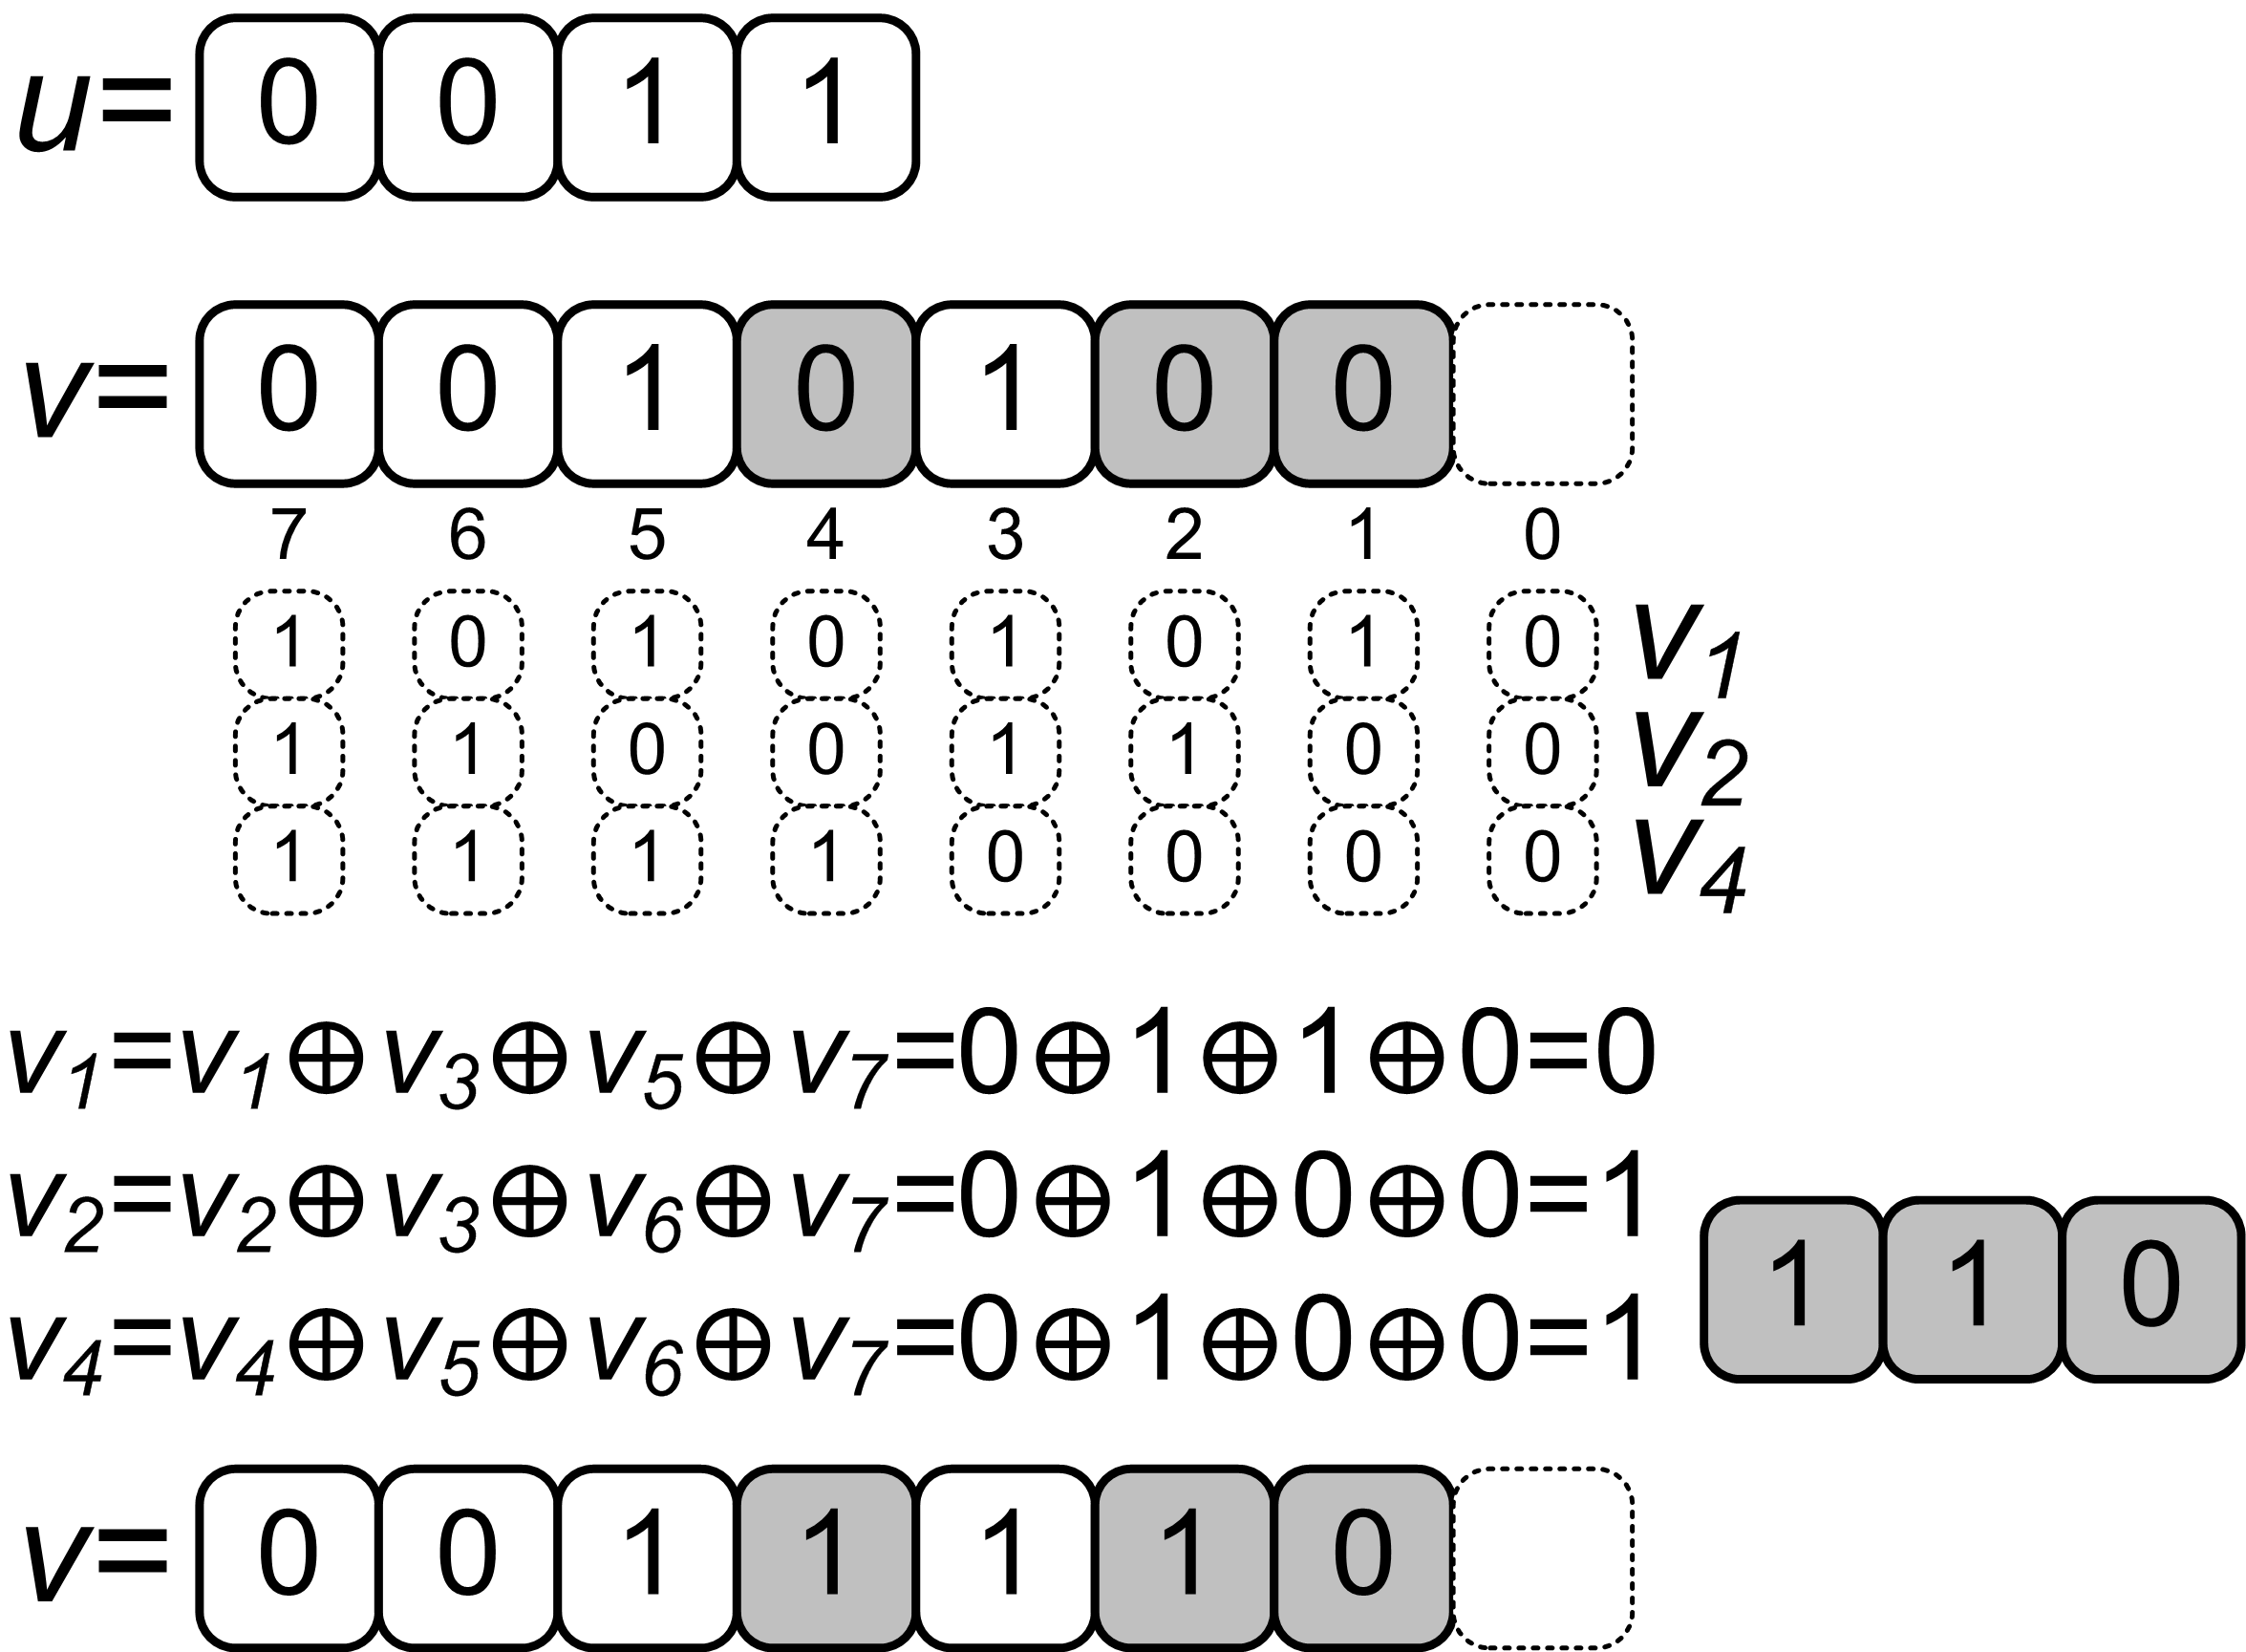
\includegraphics[width=0.6\textwidth]{fig/hammingEncode}
    \end{center}
\end{frame}

\begin{frame}
    \frametitle{Код Хемминга}
    \framesubtitle{Обнаружение и исправление одиночных ошибок}
    
    \begin{center}
        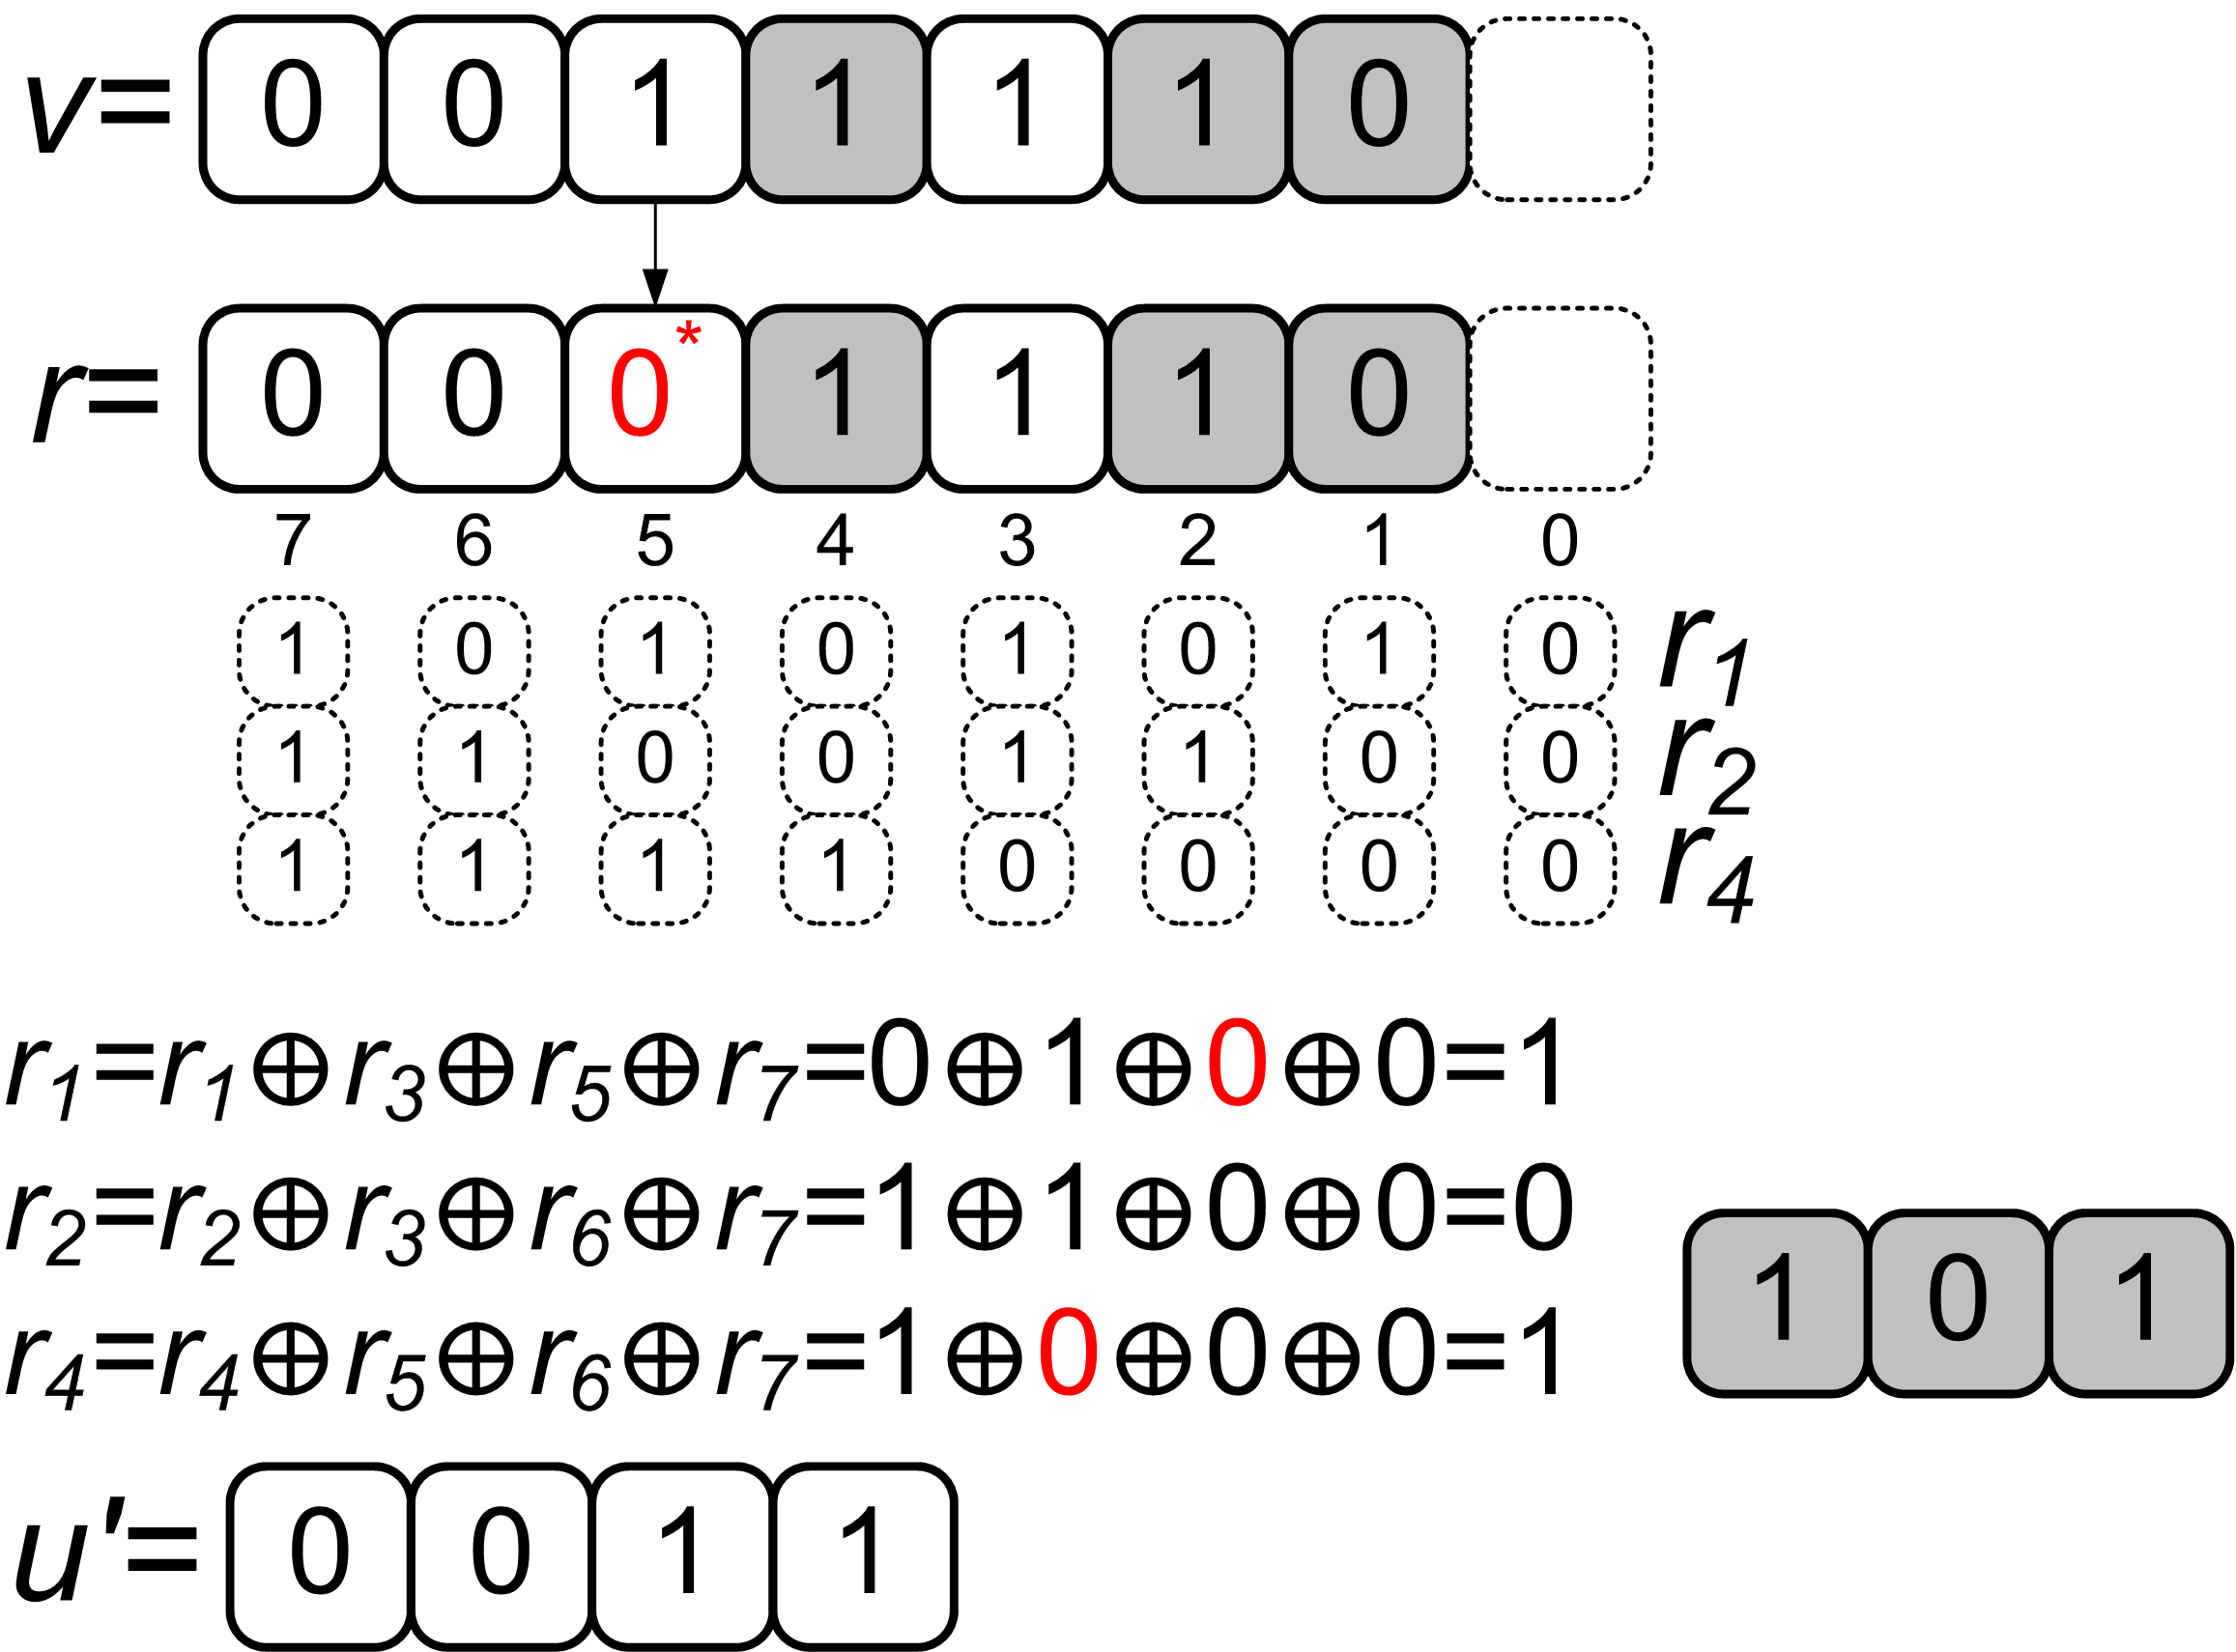
\includegraphics[width=0.6\textwidth]{fig/hammingDecode}
    \end{center}
\end{frame}

\begin{frame}
    \frametitle{Код Хемминга}
    \framesubtitle{Задание}
    
    Получена последовательность бит $r$. Перед передачей из исходного 4-х битного слова был получен код Хемминга. Выяснить, были ли ошибки в процессе передачи. Если были, то выполнить коррекцию, предполагая, что ошибка одиночная. Выделить исходное 4-х битное слово.
    \begin{center}
        \only<1>{ 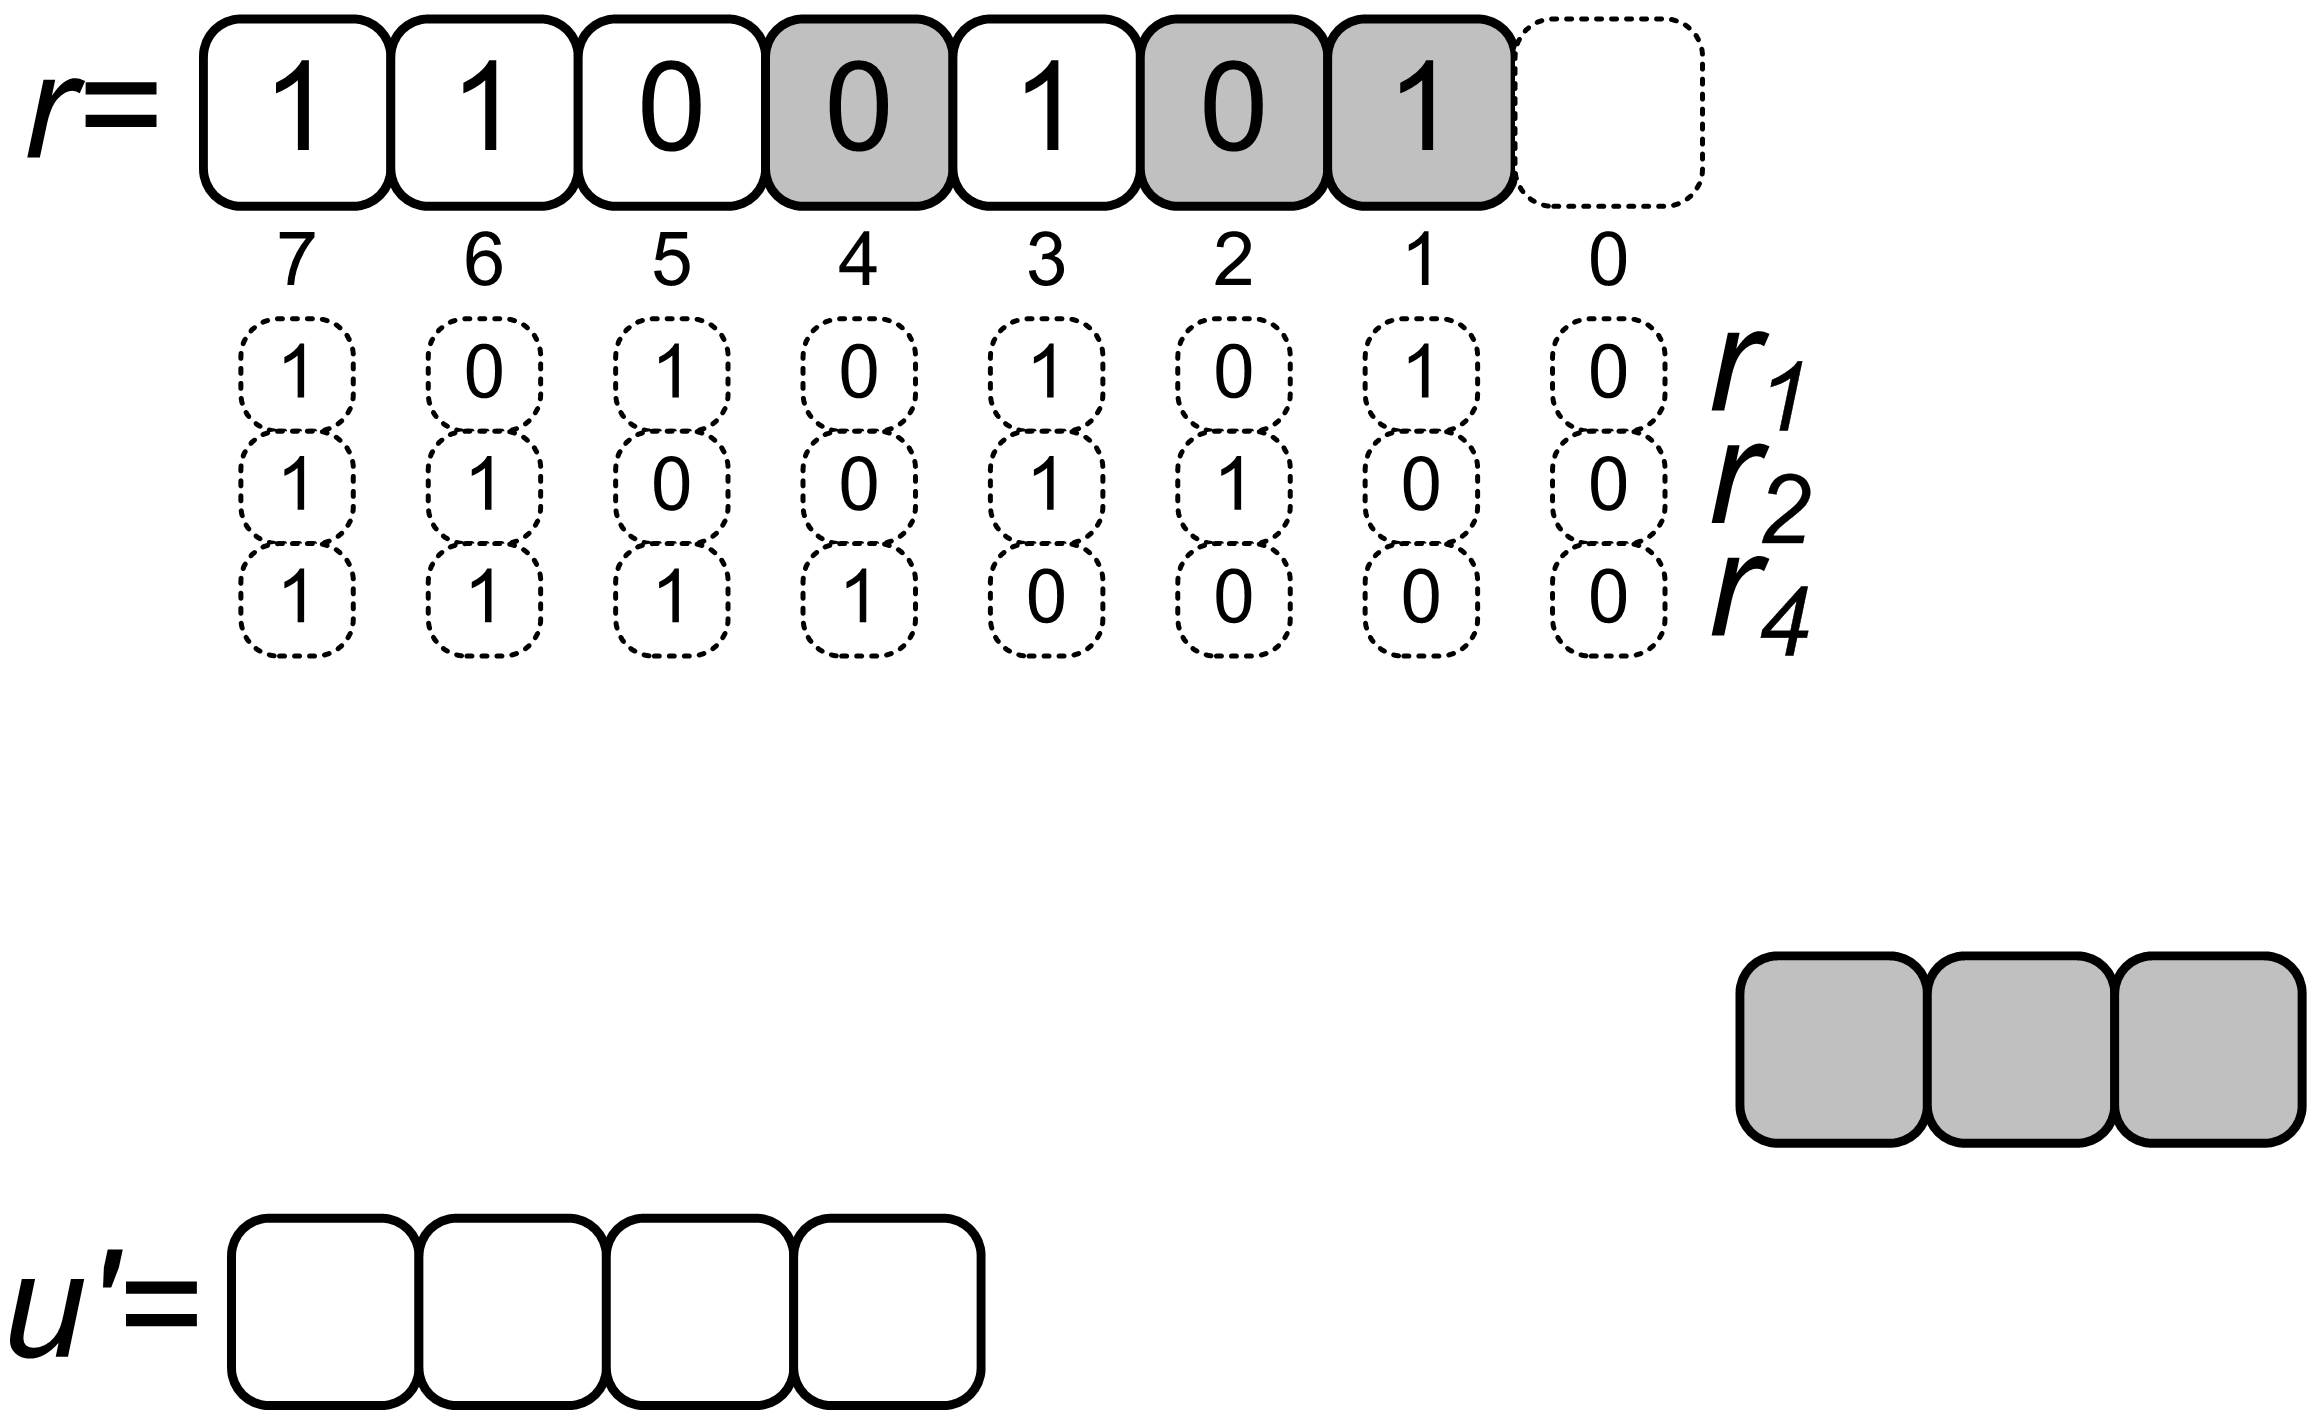
\includegraphics[width=0.6\textwidth]{fig/hammingTask} }
        \only<2>{ 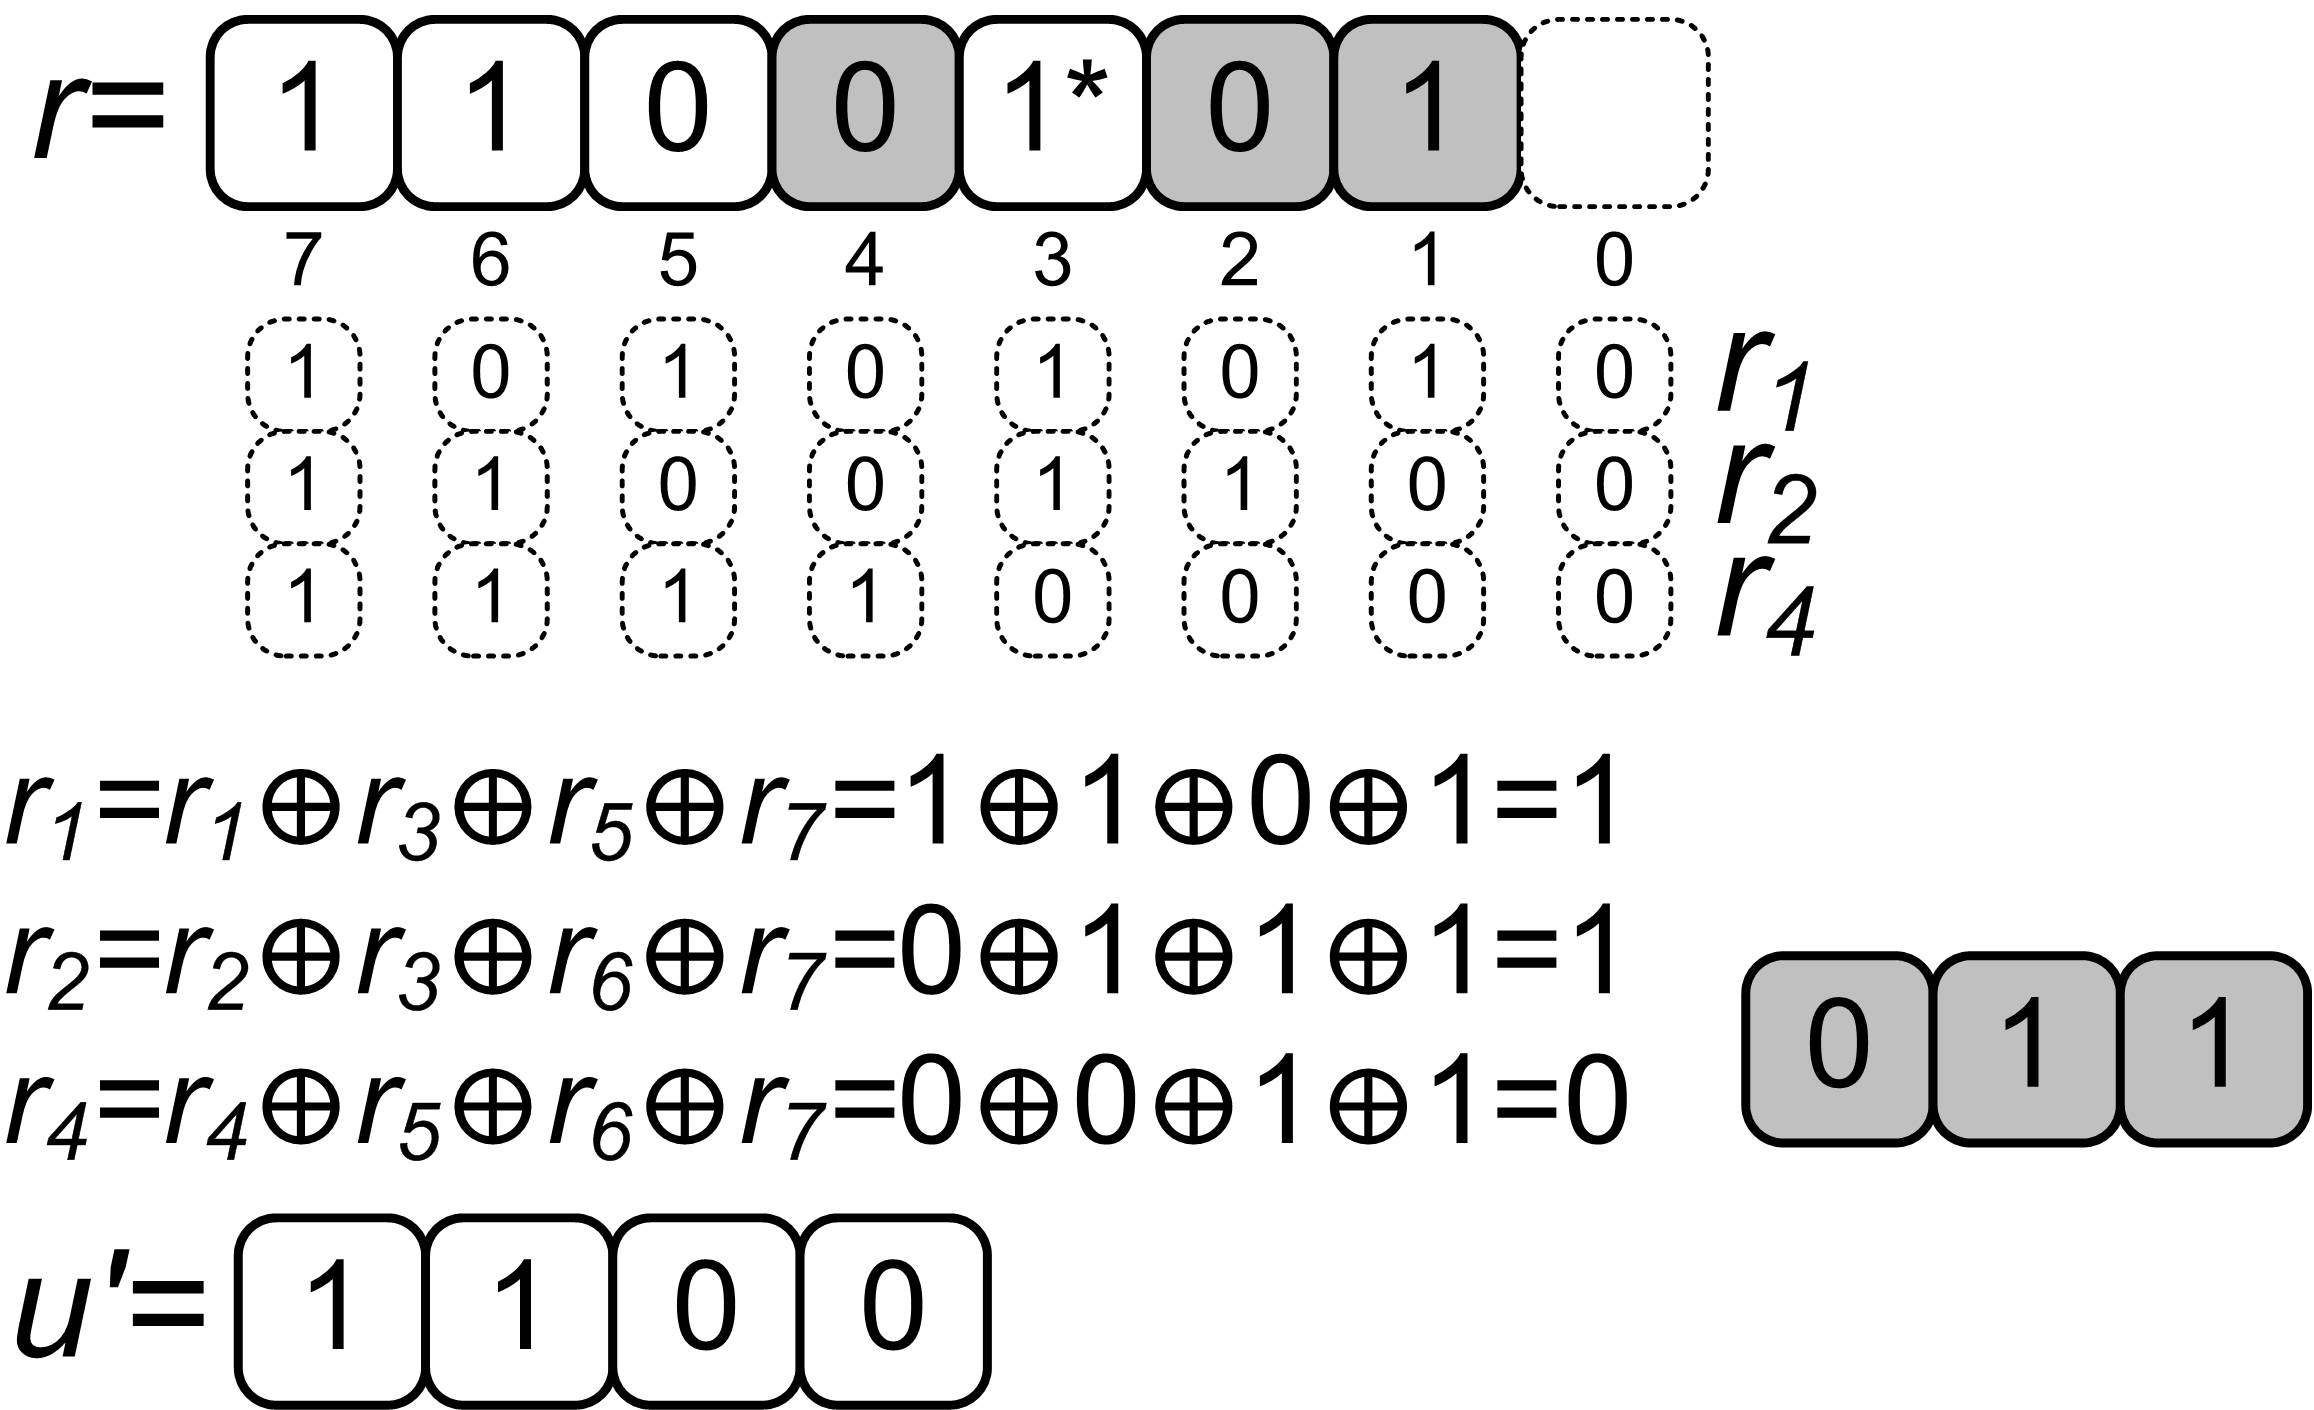
\includegraphics[width=0.6\textwidth]{fig/hammingAnswer} }
    \end{center}
\end{frame}    


\appendix


\begin{frame}
    \frametitle{В заключение}
    
    Изложение  математических основ кодирования можно найти, например, в \cite{bib:novic:discrmathprogrammer,bib:yablonsky:discreteintro}. По основам теории информации можно рекомендовать книгу \cite{bib:panin:informationTheory}. Основы кодирования подробно изложены в \cite{bib:verner:codingBase}. Заинтересовавшимся алгоритмами сжатия можно рекомендовать книгу \cite{bib:salmon:compressing}.
\end{frame}


\begin{frame}[allowframebreaks]{Библиография}
    \bibliographystyle{gost780u}
    \bibliography{./../../bibliobase}
\end{frame}

\end{document}